\documentclass[11pt,a4paper]{article}
\usepackage[T1]{fontenc}
\usepackage[utf8]{inputenc}
\usepackage[british]{babel}
\usepackage[margin=25mm]{geometry}
\usepackage{amsmath,amsthm}
\usepackage{newtxtext,newtxmath}
\usepackage{microtype}
\usepackage{booktabs,tabularx}
\usepackage[round,authoryear]{natbib}
\usepackage{pgfplots}
\usepgfplotslibrary{fillbetween,groupplots}
\pgfplotsset{compat=1.18}
\usepackage{xcolor}
\definecolor{policyblue}{HTML}{245D8F}
\definecolor{newsorange}{HTML}{BA5B21}
\usepackage[colorlinks=true,linkcolor=policyblue,citecolor=policyblue,urlcolor=policyblue]{hyperref}
\hypersetup{pdflang={en-GB},pdftitle={Policy and information news in German consumer-goods production},pdfauthor={Amanjeet Singh},pdfcreator={Amanjeet Singh},pdfsubject={Monetary economics and matched production projections},pdfkeywords={Monetary policy; information shocks; consumer-goods production; local projections}}
\newtheorem{proposition}{Proposition}
\newcounter{mainsections}
\AtEndDocument{\clearpage
  \typeout{Manuscript pages: \number\numexpr\value{page}-1\relax}
  \ifnum\value{page}>21\relax
    \PackageError{manuscript}{Twenty-page limit exceeded}{Shorten the manuscript, including appendices and references.}
  \fi}
\newcommand{\E}{\mathbb{E}}
\newcommand{\Var}{\operatorname{Var}}
\newcommand{\Cov}{\operatorname{Cov}}
\setlength{\parindent}{1.3em}
\setlength{\parskip}{0pt}
\AtBeginDocument{\setlength{\abovedisplayskip}{8pt plus 2pt minus 2pt}
 \setlength{\belowdisplayskip}{8pt plus 2pt minus 2pt}}
\setlength{\emergencystretch}{1em}
\interfootnotelinepenalty=10000
\title{Policy and information news in\\German consumer-goods production}
\author{Amanjeet Singh}
\date{11 October 2026}
\begin{document}
\maketitle
\begin{abstract}
I examine how separating policy and information contributions to ECB announcements changes the German consumer-goods durability contrast. Matched local projections on 308 monthly origins give a twelve-month policy contrast of $-2.29$ percentage log-change points per ten-basis-point factor contribution, compared with $-1.03$ for recomposed news. The exact $1.26$ adjustment has prespecified conservative 95 per cent bounds $[-0.11,3.31]$. Joint construction and period comparisons do not establish tight equivalence. Across every financially admissible rotation of the retained factor, the point gap ranges from $0.02$ to $9.01$; a common conditional 95 per cent sampling envelope includes zero. A stock-flow benchmark explains possible user-cost amplification, while production measurement limits household interpretation. An explicit latent-shock sensitivity shows that the projection adjustment equals a causal adjustment only under additional separation and exogeneity assumptions. Predetermined-outcome tests do not reject but cannot verify those assumptions. The evidence supports a directionally stable point comparison within this rotation family, rather than a precise, construction-invariant causal effect.
\end{abstract}

\noindent\textit{Keywords:} monetary policy; information shocks; consumer-goods production; local projections
\par\smallskip\noindent\textit{JEL classification:} C22, E32, E52.
\section{Introduction}
\label{sec:intro}

Monetary-policy announcements can change expectations about both financing conditions and the economic outlook \citep{JarocinskiKaradi2020}. An unexpected rise in near-term rates may signal tighter policy, favourable information about activity, or both. I ask how separating these current announcement contributions changes the estimated response of German durable relative to non-durable consumer-goods production. The economic problem is that a smaller coefficient on combined news need not imply weaker policy transmission: the measured announcement mixture can change the apparent durability contrast.

Durability makes this comparison economically meaningful. A stock supplies services after purchase, allowing replacement expenditure to adjust more than current services. Its user cost depends on financing, expected resale prices and risk; income and wealth news can also change purchases. These mechanisms can produce different relative responses to policy and information contributions, but relative prices and firms' financing can alter the ordering \citep{BarskyEtAl2007,DuranteEtAl2022,DedolaLippi2005}. German production additionally serves exports and inventories. I therefore use household theory to organise possible transmission mechanisms while estimating a defined production contrast.

I compare projections on separated contributions with a projection on their recomposed rate factor, holding production outcomes, origin months, controls and rate units constant. Both already condition on decomposed announcement histories, so the comparison isolates the current contribution conditional on those histories. The primary object is the recomposed coefficient less the policy-component coefficient at twelve months. Established partial-regression algebra decomposes this gap into a controlled information weight and the component-response difference. The weight is a covariance ratio, not an announcement probability. Its sampling variation and covariance with the response difference enter population inference.

The policy-component point contrast is $-2.29$ percentage log-change points per ten-basis-point contribution to the supplied factor, compared with $-1.03$ for recomposed news. The $1.26$ adjustment has prespecified conservative 95 per cent bounds $[-0.11,3.31]$. A supplementary zero-product test rejects for the selected median construction, but not for the alternative construction or earlier period. Joint comparisons distinguish failure to reject a difference from evidence of equivalence. More importantly, the complete financially admissible rotation family gives point adjustments between $0.02$ and $9.01$, despite keeping the outcome, historical control span and rate normalisation fixed. Its common conditional sampling envelope includes zero.

My project-specific argument concerns how the ranking of relative responses and the measurement of announcement news jointly determine the adjustment. A positive gap need not mean that information news expands relative durable production. For a latent policy intervention, I state the separation and exogeneity assumptions under which the measured gap equals its causal adjustment. Existing research establishes durability heterogeneity and information-adjusted shocks; neither combining these methods nor the algebra alone is a new theoretical contribution. Section~\ref{sec:economic-context} develops the economic mechanism; Sections~\ref{sec:data_measurement}--\ref{sec:uncertainty} define measurement and inference; Sections~\ref{sec:evidence}--\ref{sec:extension} assess the evidence and identification; Section~\ref{sec:interpretation} interprets the findings.

\section{Economic rationale and related evidence}
\label{sec:economic-context}

\subsection{Durability, purchases and production}

A durable purchase adds to a stock that supplies services over time; expenditure and service consumption are distinct objects \citep{Mankiw1982,BarskyEtAl2007}. I use a simple benchmark to separate user-cost and demand channels, rather than to calibrate a German production elasticity. With non-durable consumption $C_t$ as numeraire, end-of-period stock $S_t$, purchases $X_t$ and depreciation $0<d\le1$,
\begin{equation}
 S_t=(1-d)S_{t-1}+X_t.\label{eq:stock-law}
\end{equation}
For an interior household with logarithmic utility weights $\alpha$ and $1-\alpha$, the stock-service condition is
\begin{equation}
 \frac{S_t}{C_t}=\frac{1-\alpha}{\alpha q_t},\qquad
 q_t=p_t-(1-d)\E_t[M_{t+1}p_{t+1}]>0.
 \label{eq:user-cost}
\end{equation}
Here $p_t$ is the durable price in non-durable units and $M_{t+1}$ the household's marginal-utility discount factor. User cost deducts the risk-adjusted retained resale value from today's price. Holding current and expected relative prices and the risk-adjustment term fixed, a higher real financing rate raises user cost when $d<1$; the financing effect vanishes at $d=1$. Expected resale prices and risk can offset the cost movement, while income and wealth can change the purchase response through $C_t$. Appendix~\ref{app:household} derives the conditions and states the required interiority, resale and timing assumptions.

At a stationary-stock base with positive replacement purchases $\bar X=d\bar S$, holding inherited stock fixed gives the local relation
\begin{equation}
 \mathrm d\log(X_t/C_t)=\left(\frac1d-1\right)\mathrm d\log C_t
                  -\frac1d\mathrm d\log q_t.
 \label{eq:relative-flow}
\end{equation}
The stock-flow ratio $1/d$ amplifies the purchase adjustment needed to change services. Conditional on current non-durable consumption, a user-cost increase reduces the relative purchase flow; favourable demand or wealth news can act in the opposite direction when $d<1$. These are local partial responses. Adjustment costs, borrowing constraints and endogenous relative prices can alter them. In the general-equilibrium models of \citet[pp.~990--992, 995]{BarskyEtAl2007}, which sector has sticky prices can even reverse durable co-movement with a monetary expansion. Their long-lived-durable argument does not supply an unconditional ordering for these production groups.\footnote{The simple US expenditure dynamics tested by \citet{Mankiw1982} are rejected; I use its stock-service distinction as a conceptual foundation, not empirical validation. The benchmark's real return is period-matched to depreciation. The empirical OIS factor is nominal and annualised, so inserting its ten-basis-point contribution into the household derivative would require an additional mapping.}

The mechanism motivates heterogeneity without predicting the sign of the information-component durable-minus-non-durable response. Favourable news can raise both sectors equally, or raise non-durable activity more. A positive adjustment gap requires an information response above the policy response when the weight is positive; it does not require a positive relative information response. \citet{DuranteEtAl2022} provide firm-level evidence of stronger investment and sales responses among durable producers, while the household benchmark explains one reason the purchase flow can be sensitive.

Production can respond through domestic purchases, foreign demand, inventories and firms' financing. Sales and output need not move together. \citet{DedolaLippi2005} relate industrial responses to financing requirements, borrowing capacity and firm size as well as durability. A production contrast therefore combines demand and supply adjustments rather than estimating a household-demand elasticity. The official grouping is also consequential: motor vehicles are capital goods, and non-durable production excludes services.\footnote{Regulation (EU) 2020/1197, Annex II.A, governs production allocation. The supply-use manual includes motor vehicles in household consumer durables \citep[pp.~151, 397]{Eurostat2008}. These are distinct measurements.}



The published production evidence already establishes heterogeneous transmission. \citet{PeersmanSmets2005} study eleven industries in seven euro-area countries over 1980--1998, including capital and intermediate durables. \citet{DedolaLippi2005} examine twenty-one sectors in five countries using domestic-policy identification. Both include Germany. \citet{ChoiEtAl2024} use annual international industry interactions \citep[\S\S~III--IV]{ChoiEtAl2023}; their approach recognises that common macroeconomic disturbances can load differently across sectors. Differencing removes an identical common response, not every common disturbance.

\subsection{Information adjustment and the economic comparison}

An interest-rate surprise around a policy announcement can convey more than an unexpected change in the policy stance. Under the interpretation developed by \citet{JarocinskiKaradi2020}, policy tightening raises the rate surprise while lowering equity prices, whereas favourable central-bank information can raise both. The latter component may affect expected activity differently from the policy component. A regression on their combined rate contribution can consequently describe a different production response from a regression that separates them. In this study, the same supplied factor provides the rate units for both comparisons; its contribution is not an equal-sized change in a particular ECB policy rate.

The labels remain identifying interpretations. \citet{BauerSwanson2023a} show that an unexpectedly strong systematic policy response to public news can retain conventional rate--equity signs. Their Fed evidence challenges identification rather than measuring ECB contamination. Their monthly LP-IV analysis also has a different intervention normalisation \citep{BauerSwanson2023b}. I therefore do not equate the information contribution with superior private knowledge or identify its production response as an expectations channel.

Information-adjusted durability comparisons are established. \citet{DuranteEtAl2022} combine firms in four euro-area economies with original poor-man ECB shocks; their annual investment and sales outcomes cover broader manufacturing groups. \citet{CasalisKrustev2022} compare quarterly expenditure, including non-durable services, using broader monetary and credit conditions \citep[\S\S3.1, 4.2]{CasalisKrustev2020}. These outcomes, categories and interventions differ from my matched monthly production comparison.

A closely related working paper by \citet{FlaccadoroRopele2026} combines monthly euro-area consumer-goods production, information-adjusted ECB shocks and local projections. Its broad-durability comparison and coarse two-digit consumer-group mapping differ from my detailed official allocation. This unpublished June 2026 supplement rules out treating that combination of methods as a contribution by itself. I focus on the matched current-announcement gap conditional on shared histories, rather than claim historical priority for the exact contrast.

\section{Data and measurement}
\label{sec:data_measurement}

I use German monthly production-volume indices for durable and non-durable consumer goods from Eurostat's \texttt{sts\_inpr\_m} dataset. Both indices are seasonally and calendar adjusted and referenced to 2021=100. They measure production in the official main industrial groupings (MIGs). These groupings combine NACE Rev.~2 divisions and groups, rather than assigning every two-digit manufacturing industry to a durability category \citep{EC2020,Eurostat2026}. Consumer durables comprise consumer electronics, optical and photographic equipment, domestic appliances, miscellaneous transport equipment, furniture, jewellery and musical instruments. Crucially, motor-vehicle manufacturing belongs to capital goods.\footnote{The durable grouping contains NACE Rev.~2 groups 26.4, 26.7, 27.5 and 30.9, division 31, and groups 32.1 and 32.2. Division 29, including motor vehicles, trailers and semi-trailers, is allocated to capital goods in Regulation 2020/1197, Annex II.A. Short-term statistics retain NACE Rev.~2 through 2027.} I therefore interpret the outcome as relative production in these defined manufacturing groupings. Exports, inventories and financing can influence production alongside domestic household demand; the indices do not separately identify these channels.

My price control uses Germany's unadjusted all-items HICP, \texttt{prc\_hicp\_midx}, in the historical ECOICOP classification, referenced to 2015=100. I construct annual logarithmic inflation as
\begin{equation}
  \pi_t=100\log\!\left(P_t/P_{t-12}\right).
  \label{eq:annual_inflation}
\end{equation}
HICP ends in December 2025; the last required lag is July 2025 at the final primary origin. Production extends to August 2026, and future prices are unnecessary. I retain one coherent historical HICP classification.\footnote{The successor \texttt{prc\_hicp\_minr} uses ECOICOP version 2; I do not splice it into this series. Month indicators do not make HICP officially seasonally adjusted.} Constant rebasing cancels in log changes.

The announcement variables are an author-maintained update of the policy and information decomposition introduced by \citet{JarocinskiKaradi2020}, using the EA-MPD monetary-event window of \citet{AltavillaEtAl2019}. I fix the update to its 7 January 2026 revision \citep{JarocinskiUpdate2026}. Its near-term rate factor is the first principal component of one-, three- and six-month and one-year OIS surprises. The four inputs are standardised by their sample standard deviations, without subtracting their sample means before component extraction. The component is then scaled to the standard deviation of the one-year OIS surprise and expressed in annualised percentage points. The accompanying equity surprise is 100 times the logarithmic change in the Euro Stoxx~50.

I use the supplied median admissible rotation of this rate--equity system. A common selected angle applies across announcements and permits policy and information contributions within the same event \citep{Jarocinski2022,JarocinskiUpdate2026}. Their sum reconstructs the rate factor. This is a later point-selected implementation, rather than the original article's monthly implementation. Event-column orthogonality is not preserved automatically by monthly aggregation, control residualisation or sample trimming.\footnote{The code's orthogonality concerns uncentred column products; it does not establish zero centred covariance or independence.} Consequently, it cannot justify suppressing joint policy--information dependence in the empirical comparison. I divide both contributions by 0.10, so a unit change represents ten basis points of the normalised factor contribution. This normalisation does not equate the estimates with the effect of an actual ten-basis-point ECB policy-rate increase.

The supplied monthly columns equal retained event sums to recorded numerical precision. I retain zero-event months and leave dates outside coverage missing. The primary sample has 308 origins; the common response-path sample has 296 through August 2024. The October retrieval contains revised historical data rather than real-time announcement information. Appendix~\ref{app:source_reconciliation} records reconciliation; numerical consistency does not establish identification.


Table~\ref{tab:variation} puts the reporting scale in context. A ten-basis-point factor contribution is approximately three sample standard deviations of monthly policy news, rather than a typical announcement-size assumption. The primary calendar retains 45 months without source events. Durable and non-durable monthly growth have sample standard deviations of $3.85$ and $1.89$ percentage log-change points, respectively; these describe production variability, rather than policy responses.

% BEGIN VARIATION_TABLE
\begin{table}[htbp]
\centering\small
\caption{Monthly announcement variation on the primary origins}
\label{tab:variation}
\begin{tabular}{@{}lrr@{}}
\toprule
Contribution & Sample SD, basis points & Control-residual SD, basis points \\
\midrule
Policy contribution & $3.32$ & $2.77$ \\
Information contribution & $2.79$ & $2.41$ \\
Recomposed factor & $4.35$ & $3.59$ \\
\bottomrule
\end{tabular}
\par\smallskip\begin{minipage}{.97\textwidth}\footnotesize
January 2000--August 2025, $n=308$, including 45 months without retained events. Both columns use divisor $n-1$. The right column removes the same 72 controls defined in Section~\ref{sec:design} from each current contribution, without removing the other current component. These are descriptive standard deviations in normalised factor units, not disturbance standard errors or actual policy-rate changes.
\end{minipage}
\end{table}
% END VARIATION_TABLE

\section{Matched empirical design}
\label{sec:design}

\subsection{Outcome and announcement units}

Let $D_t$ and $N_t$ denote strictly positive durable and non-durable production indices. For each horizon $h$, I use
\begin{equation}
 Y_{t,h}=100\left\{\log\frac{D_{t+h}}{N_{t+h}}-\log\frac{D_{t-1}}{N_{t-1}}\right\}.
 \label{eq:outcome}
\end{equation}
This is the difference between the two cumulative percentage log changes, rather than a ratio of physical production quantities. It is invariant to separate constant rebasing of the indices. At $h=12$, the endpoint is one year after the announcement month relative to the preceding month, so the outcome sums thirteen monthly changes. I estimate these cumulative responses using local projections \citep{Jorda2005,StockWatson2018}. Section~\ref{sec:uncertainty} develops the inference for the matched coefficient comparison.

Write $m_t=m_t^{\rm raw}/0.10$ and $c_t=c_t^{\rm raw}/0.10$ for the supplied policy and information contributions, and recompose $r_t=m_t+c_t$. All three regressors share rate-factor units. A unit is a ten-basis-point contribution to the normalised factor, not an observed policy-rate intervention of that size. I do not independently standardise the two components, since that would alter the comparison's units and its decomposition.

\subsection{Controls, sample and comparison}

I estimate the two ordinary least-squares projections
\begin{align}
 Y_{t,h}&=\beta_{m,h}m_t+\beta_{c,h}c_t+Z_t^\top\eta_h+e_{t,h},\label{eq:full}\\
 Y_{t,h}&=\gamma_h r_t+Z_t^\top\zeta_h+v_{t,h}.\label{eq:reduced}
\end{align}
The same rows and $Z_t$ enter both. They define linear-projection coefficients; the equations do not, by themselves, establish a correctly specified conditional mean or a structural intervention. A structural reading needs more. In a noiseless benchmark, let the supplied components $s_t=(m_t,c_t)^\top$ measure latent innovations $\varepsilon_t$ through a constant invertible matrix $A$, and let the structural relative response be $b_h$. Conditional orthogonality of the remaining production disturbance to the measured components then gives
\begin{equation}
 s_t=A\varepsilon_t,\qquad \beta_h=A^{-\top}b_h,
 \quad \beta_h=(\beta_{m,h},\beta_{c,h})^\top.
 \label{eq:measurement-bridge}
\end{equation}
Appendix~\ref{app:causal-bridge} proves this relation. A known diagonal mapping recovers the separately scaled latent responses. An unknown dense mapping mixes them; measurement noise generally breaks this identity. Orthogonal observed columns do not establish a diagonal mapping, exogeneity or response invariance. Rate--equity restrictions select an admissible interpretation of announcement news, rather than prove these conditions. I therefore estimate supplied-component projections and state the stronger assumptions needed to call them causal responses \citep{JarocinskiKaradi2020,StockWatson2018}.

The controls are an intercept, eleven calendar-month indicators and twelve lags each of durable growth, non-durable growth, annual HICP log inflation and both scaled announcement components. Preceding reference months avoid contemporaneous production controls; month indicators allow residual seasonal and announcement-opportunity patterns. Twelve lags admit a year of history, while the matched six-lag check assesses parameter cost. These histories define conditioning, not a proven sufficient information set. Both models retain decomposed histories, so the primary gap concerns current separation rather than abandoning information adjustment at every date.

The full primary regression has 74 columns and 234 residual degrees of freedom. Origins require current components, complete lag histories, and positive production at $t-1$ and $t+h$, without imputation or primary pandemic exclusions. Future prices and shocks are unnecessary. The August 2026 production endpoint gives 308 twelve-month origins, January 2000--August 2025. Pooling different policy regimes and pandemic states does not establish a stable structural response. Appendix~\ref{app:record} records the specification chronology and declared checks.

The primary horizon, dates, outcome, units, controls and interval were fixed before response fitting. Direct regressions on supplied contributions have no IV first stage; small residual variation and influential announcements concern projection precision rather than weak-instrument statistics \citep{StockWatson2018}.

The primary adjustment gap and the component-response difference are
\begin{equation}
 \delta_h=\gamma_h-\beta_{m,h},\qquad
 \theta_h=\beta_{c,h}-\beta_{m,h}.
 \label{eq:gap}
\end{equation}
The policy coefficient is a companion estimand. Neither its individual interval nor the information coefficient's interval replaces an interval for $\delta_h$.

\begin{proposition}[Matched rate-surprise comparison]
\label{prop:mixture}
On identical rows, controls and units, let $Z$ have full column rank, $[m,c,Z]$ have full rank and $n>\operatorname{rank}[m,c,Z]$. Then
\begin{equation}
 \widehat\delta_h=\widehat w_{c,h}\widehat\theta_h,
 \qquad \widehat w_{c,h}=
 \frac{r^\top M_Zc}{r^\top M_Zr},\qquad
 M_Z=I-Z(Z^\top Z)^{-1}Z^\top.
 \label{eq:sample-gap}
\end{equation}
\end{proposition}

This application of the partial-regression result reviewed by \citet{Ding2021} is proved in Appendix~\ref{app:sample}. Its economic interpretation is straightforward. If the information weight is positive and the information response exceeds the policy response, combining the components shifts the estimated coefficient upward. When the policy response is negative, this makes the relative contraction appear smaller. But the weight need not lie in $[0,1]$: it reflects controlled covariation, rather than a probability or a variance share. Monthly aggregation, conditioning and horizon trimming can change that covariation even when the event-level source construction is orthogonal.

\section{Uncertainty in the adjustment gap}
\label{sec:uncertainty}

For population inference, $w_c$ is a residualised moment ratio and varies with the regressor sample. Conditioning on a supplied factor and rotation does not fix this estimated weight.

Under regular joint asymptotic linearity, the gap's influence satisfies
\begin{equation}
 \psi_{\delta,t}=w_c\psi_{\theta,t}+\theta\psi_{w,t},
 \label{eq:main-influence}
\end{equation}
with horizon subscripts suppressed. Thus its variance includes component-response variation, weight variation and their covariance. Appendix~\ref{app:population} derives each term, including the effect of residualising on estimated controls. Using only $|\widehat w_c|\operatorname{SE}(\widehat\theta)$ omits the latter two terms under alternatives; it does not establish conditional coverage by itself. At $w_c=0$ but $\theta\ne0$, weight variation is the leading first-order term. At $w_c=\theta=0$, the product gradient vanishes and ordinary gap-Wald inference is not generally regular.

I fit the full and reduced regressions with their own residuals, alongside the projection of $c$ on $[r,Z]$ that estimates $w_c$. I retain their joint coefficient contributions and cross-model covariance. The covariance uses Bartlett weights at actual calendar distances, bandwidth
\begin{equation}
 L_h=h+\left\lceil4(n/100)^{2/9}\right\rceil,
 \label{eq:main-bandwidth}
\end{equation}
and one common multiplier $n/(n-k_F)$, where $k_F$ is the full model's column count. At the primary horizon, $L_{12}=18$. The bandwidth grows with sample size; the correction is a finite-sample convention, rather than a guarantee of unbiased covariance or exact coverage. I use normal critical values and no prewhitening.

At a fixed horizon and fixed regressor dimension, I maintain positive-definite limits for each regression's moment matrix, an asymptotically linear joint coefficient expansion with a finite Gaussian score limit, and consistency of the calendar-HAC covariance estimator. These conditions require adequate moments and weak dependence, allowing the appropriate periodic moment limits for the calendar controls. The declared bandwidth satisfies $L_h\to\infty$ and $L_h/n\to0$, while $n/(n-k_F)\to1$. These rate properties do not establish covariance consistency in the retained data. Structural breaks, arbitrary trends and influential observations can invalidate the approximation; uncorrelated surprises do not imply uncorrelated projection scores with overlapping outcomes. The lag-augmentation result of \citet{MontielOleaPlagborgMoller2021}, with its corrected assumptions \citep{MontielOleaPlagborgMoller2026}, requires state lags and innovation conditions that my constructed-shock design does not establish automatically.

For the primary comparison I use a conservative product interval. I form individual 97.5 per cent normal intervals for $w_c$ and $\theta$, with critical value $z_{0.9875}$, and take the smallest and largest of their four endpoint products. The Bonferroni union bound gives asymptotic joint coordinate coverage of at least 95 per cent; mapping that rectangle covers their product. Appendix~\ref{app:covariance} proves the coverage statement. It avoids requiring an invertible joint covariance or a regular product gradient, while retaining the need for valid, nondegenerate marginal inference. I do not clip weights to $[0,1]$. The null $\delta_h=0$ is the union of $w_{c,h}=0$ and $\theta_h=0$. The declared rectangle is deliberately conservative; its non-rejection does not imply agreement among all valid zero-gap tests. Under a maintained nonzero weight, a restricted-null test of $\theta_h=0$ has a different justification. The preselected product interval remains primary. Section~\ref{sec:gap-followup} reports supplementary procedures introduced after inspection to assess the zero-product geometry.

Companion intervals are pointwise; the normal gap interval is a regularity-dependent diagnostic. The original intervals condition on the selected factor, rotation, vintage and design. Section~\ref{sec:extension} adds inference across the retained factor's full rotation set, without covering re-estimation of the factor or its sign-set boundaries.

\section{Empirical evidence}
\label{sec:evidence}

\subsection{The primary twelve-month comparison}

Table~\ref{tab:primary} reports the matched estimates. The policy-component contrast is $-2.29$, with a contextual normal interval $[-4.18,-0.40]$. The underlying sector estimates are $-3.47$ for durable production and $-1.18$ for non-durable production. Their covariance is retained in the relative response, rather than judging it from separate sector significance. The information-component contrast is $0.66$, with an interval including zero. These are cumulative log-change responses per the declared ten-basis-point factor contribution.

% BEGIN PRIMARY_TABLE
\begin{table}[htbp]
\centering\small
\caption{Primary twelve-month projections}
\label{tab:primary}
\begin{tabular}{@{}lrrl@{}}
\toprule
Quantity & Estimate & 95\% interval & Basis \\
\midrule
Durable policy response & $-3.47$ & $[-5.63,-1.31]$ & Pointwise normal \\
Non-durable policy response & $-1.18$ & $[-2.14,-0.21]$ & Pointwise normal \\
Relative policy response & $-2.29$ & $[-4.18,-0.40]$ & Pointwise normal \\
Relative information response & $0.66$ & $[-1.07,2.39]$ & Pointwise normal \\
Recomposed-rate response & $-1.03$ & $[-2.24,0.17]$ & Pointwise normal \\
Adjustment gap & $1.26$ & $[-0.11,3.31]$ & Conservative product \\
\bottomrule
\end{tabular}
\par\smallskip\begin{minipage}{.97\textwidth}\footnotesize
Origins: January 2000--August 2025, $n=308$. Responses are percentage log-change points per ten-basis-point normalised factor contribution. The full model has 74 columns; Bartlett bandwidth is 18. The gap uses the prespecified product interval. Other intervals are individual normal approximations and do not give simultaneous coverage. The underlying sector coefficients retain their joint covariance.
\end{minipage}
\end{table}
% END PRIMARY_TABLE

Recomposed news gives a point response $1.26$ closer to zero than the policy contribution. This is a projection comparison, not two identical policy interventions. The prespecified conservative interval $[-0.11,3.31]$ includes zero and accommodates a substantial positive adjustment; non-rejection is not evidence of economic irrelevance.

The information weight is $0.427$ and response difference $2.951$. Their 97.5 per cent coordinate bounds are $[0.312,0.542]$ and $[-0.198,6.100]$: uncertainty in the ranking permits the negative product endpoint. The weight is a controlled covariance ratio, not a fraction of information announcements. Separate coefficient significance does not test the gap.

\subsection{Supplementary inference on the zero-gap restriction}
\label{sec:gap-followup}

After primary inspection and preliminary arithmetic, I recorded supplementary zero-product inference for all six declared cases. The intersection-union test and joint-ellipse product bounds use unchanged estimates. Appendix~\ref{app:gap-tests} gives their justification and all results; this follow-up is not prospective registration.

% BEGIN FOLLOWUP_SUMMARY
The primary intersection-union test gives $p=0.036$, a nominal 5 per cent rejection of the zero-product restriction. Its joint-ellipse product bounds are $[-0.19,3.18]$. Every joint-region interval includes zero. The poor-man and pre-pandemic tests do not reject, with $p=0.174$ and $p=0.414$. Table~\ref{tab:gap-followup} reports all six cases without selection.
% END FOLLOWUP_SUMMARY

The procedures calibrate the same restriction differently. Nominal point-null rejection for the selected decomposition does not establish a minimum economic adjustment, construction robustness or causality.

\subsection{The dynamic comparison}

Figure~\ref{fig:path} presents horizons zero to twenty-four on 296 common origins, January 2000 to August 2024. The common sample avoids letting changing origin composition alone explain differences across horizons.\footnote{At $h=0$, the outcome covers the whole announcement month, including production before the announcement; it is not an instantaneous event-window response.} Its twelve-month point gap is $1.21$, with conservative bounds $[-0.20,3.27]$; it must not replace the primary estimate based on 308 origins.

% BEGIN PATH_FIGURE
\begin{figure}[htbp]
\centering
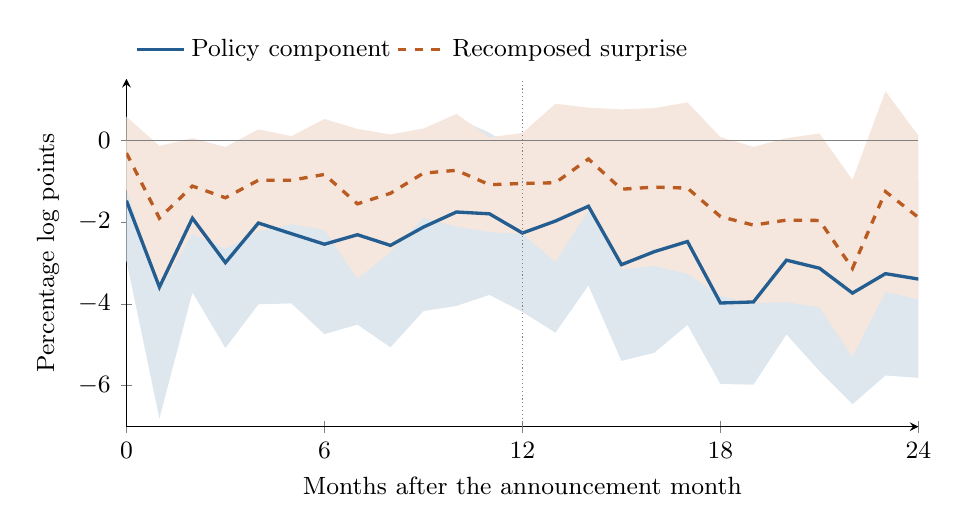
\begin{tikzpicture}
\begin{axis}[width=.96\textwidth,height=6.0cm,
 axis lines=left,xmin=0,xmax=24,xtick={0,6,12,18,24},
 xlabel={Months after the announcement month},ylabel={Percentage log points},
 tick label style={font=\small},label style={font=\small},
 legend style={at={(0,1.02)},anchor=south west,draw=none,font=\small},legend columns=2,
 clip=true]
\addplot[name path=policylo,draw=none,forget plot] coordinates {(0,-2.943122413) (1,-6.801849047) (2,-3.721363507) (3,-5.0784112) (4,-4.010344612) (5,-3.989010434) (6,-4.739972413) (7,-4.506214663) (8,-5.061940555) (9,-4.176258386) (10,-4.050481166) (11,-3.781477863) (12,-4.195359839) (13,-4.704970818) (14,-3.548597193) (15,-5.393500792) (16,-5.192751962) (17,-4.512420662) (18,-5.956593231) (19,-5.974713203) (20,-4.747566707) (21,-5.6405886) (22,-6.451412745) (23,-5.749779435) (24,-5.806710868)};
\addplot[name path=policyhi,draw=none,forget plot] coordinates {(0,-0.01429367556) (1,-0.380481459) (2,-0.09205853118) (3,-0.9070330578) (4,-0.03877774168) (5,-0.5820924412) (6,-0.3451795959) (7,-0.114724169) (8,-0.08120716358) (9,-0.07107911868) (10,0.5395384578) (11,0.1821391383) (12,-0.34298599) (13,0.7525139803) (14,0.3187706414) (15,-0.6911181407) (16,-0.2532740392) (17,-0.440527171) (18,-2.001362717) (19,-1.93166333) (20,-1.117478599) (21,-0.6164413504) (22,-1.021785956) (23,-0.7738352756) (24,-0.9811124205)};
\addplot[policyblue!15,draw=none,forget plot] fill between[of=policylo and policyhi];
\addplot[policyblue,very thick] coordinates {(0,-1.478708044) (1,-3.591165253) (2,-1.906711019) (3,-2.992722129) (4,-2.024561177) (5,-2.285551438) (6,-2.542576004) (7,-2.310469416) (8,-2.571573859) (9,-2.123668752) (10,-1.755471354) (11,-1.799669362) (12,-2.269172914) (13,-1.976228419) (14,-1.614913276) (15,-3.042309467) (16,-2.723013001) (17,-2.476473916) (18,-3.978977974) (19,-3.953188266) (20,-2.932522653) (21,-3.128514975) (22,-3.73659935) (23,-3.261807356) (24,-3.393911645)};
\addlegendentry{Policy component}
\addplot[name path=ratelo,draw=none,forget plot] coordinates {(0,-1.205493552) (1,-3.672167662) (2,-2.29302024) (3,-2.651165818) (4,-2.22115784) (5,-2.056193803) (6,-2.191569967) (7,-3.386962464) (8,-2.735957079) (9,-1.896006085) (10,-2.113289063) (11,-2.247184064) (12,-2.290778781) (13,-2.970410112) (14,-1.714577981) (15,-3.148629417) (16,-3.076358412) (17,-3.266532201) (18,-3.810051635) (19,-3.989020134) (20,-3.955074179) (21,-4.087565629) (22,-5.294105929) (23,-3.708492696) (24,-3.888498771)};
\addplot[name path=ratehi,draw=none,forget plot] coordinates {(0,0.5733657055) (1,-0.140637228) (2,0.04890874938) (3,-0.1647125961) (4,0.2641939458) (5,0.09911627298) (6,0.5167972072) (7,0.2747735203) (8,0.1388573601) (9,0.2839401298) (10,0.6410444699) (11,0.06996983424) (12,0.1751395888) (13,0.8902281229) (14,0.7936856674) (15,0.7518660965) (16,0.7826794995) (17,0.9230827554) (18,0.07606046121) (19,-0.1631058327) (20,0.04899536531) (21,0.1641835976) (22,-0.9723718233) (23,1.195143332) (24,0.108074957)};
\addplot[newsorange!15,draw=none,forget plot] fill between[of=ratelo and ratehi];
\addplot[newsorange,very thick,dashed] coordinates {(0,-0.316063923) (1,-1.906402445) (2,-1.122055745) (3,-1.407939207) (4,-0.9784819469) (5,-0.9785387652) (6,-0.8373863797) (7,-1.556094472) (8,-1.29854986) (9,-0.8060329776) (10,-0.7361222963) (11,-1.088607115) (12,-1.057819596) (13,-1.040090995) (14,-0.4604461567) (15,-1.19838166) (16,-1.146839456) (17,-1.171724723) (18,-1.866995587) (19,-2.076062983) (20,-1.953039407) (21,-1.961691016) (22,-3.133238876) (23,-1.256674682) (24,-1.890211907)};
\addlegendentry{Recomposed surprise}
\addplot[gray,thin,forget plot] coordinates {(0,0)(24,0)};
\addplot[gray,densely dotted,forget plot] coordinates {(12,-7)(12,1.5)};
\end{axis}
\end{tikzpicture}
\caption{Matched response paths. Coefficients are percentage log-change points per ten-basis-point factor contribution. Shading gives 95 per cent pointwise normal HAC intervals, not simultaneous bands. All horizons use 296 common origins, January 2000--August 2024; the primary twelve-month estimate uses the longer 308-origin sample. Appendix Table~\ref{tab:sensitivities} reports the directly assessed primary gap; overlap of these individual response bands is not a test of that gap.}
\label{fig:path}
\end{figure}
% END PATH_FIGURE

The policy point estimate is negative and the gap point estimate positive throughout the displayed path. The profiles are irregular, and every shaded interval is pointwise. Selected horizons with apparently stronger separation cannot establish path-wide significance or replace the fixed twelve-month comparison. The plot documents the estimated dynamics and their precision on this sample, rather than identifying an invariant timing mechanism across policy regimes.

\subsection{Declared sensitivity and influence}

Appendix Table~\ref{tab:sensitivities} reports every declared twelve-month sensitivity. Six lags give a gap of $1.17$ with conservative bounds $[-0.16,3.13]$. Poor-man components give $1.23$ with bounds $[-1.02,4.19]$. Their close full-sample point gaps mask different component precision: the information standard error rises from $0.88$ to $2.11$, and the response-difference standard error from $1.40$ to $2.69$. Residual information variation after controls and the other component falls by about 28 per cent. Different significance labels are consequently not a direct test of construction stability.


Requiring endpoints by December 2019 gives 228 origins through December 2018. The gap falls to $0.66$ and the information contrast to $-0.62$; the policy interval $[-4.28,0.11]$ includes zero. This positive gap with a negative information contrast illustrates response ranking. The historical target and policy composition change together, so the comparison cannot isolate a pandemic effect. Bandwidths 15 and 24 leave primary coefficients unchanged and conservative gap bounds including zero.



Single-origin deletions keep the primary gap positive, but omitting December 2015 changes it by $0.38$, approximately thirty per cent. Pandemic origins are also influential. Maximum leverage is $0.565$ and the column-scaled condition number about $49.1$, with control/full/reduced ranks 72/74/73. Full rank and the multiplier $308/234$ do not correct leverage-dependent residual shrinkage or establish finite-sample coverage.\footnote{Deleting one origin does not remove its announcement from later histories or its production months from other overlapping outcomes. This is an influence diagnostic, without automatic exclusions.}

\subsection{An illustration of omitted variance terms}

Multiplying the component-difference standard error by the realised weight gives a standard error of $0.6005$ and an illustrative normal interval $[0.08,2.44]$. Retaining weight variation and cross-model covariance gives a stacked standard error of $0.6749$ and a regularity-dependent normal diagnostic interval $[-0.06,2.58]$. The primary conservative interval remains $[-0.11,3.31]$.

The variance terms are $0.3606$ for component-response uncertainty, $0.0229$ for weight variation and $0.0719$ for cross covariance, totalling $0.4554$. The latter two are 20.8 per cent of the total, but their signs are sample-specific. Dropping them from random-design variance does not establish fixed-design coverage. The six-lag standard error is 9.8 per cent smaller, but changes the conditioning set and still leaves the conservative gap interval including zero. Smoothing response paths can exchange variance for bias \citep{BarnichonBrownlees2019}; its efficiency advantage does not validate inference for this nonlinear gap or supply exogeneity. I retain the declared estimator rather than count a smaller standard error under added restrictions as resolution.

\section{Construction, period and causal identification}
\label{sec:extension}

\subsection{Joint stability and the meaning of equivalence}

I recorded this extension after the original results were known, but before calculating its new contrasts. I retain the primary evidence. For each comparison, I jointly estimate $(w_1,\theta_1,w_2,\theta_2)$, embed each equation's coefficient contributions on the same monthly calendar, and retain cross-equation covariance. Nested period samples therefore share uncertainty. A common Bartlett bandwidth 18 and each design's own $\sqrt{n/(n-k_F)}$ scaling give a positive-semidefinite joint covariance; bandwidth 17 is a declared check. I map the four-coordinate 95 per cent Wald ellipsoid through $w_2\theta_2-w_1\theta_1$, avoiding reliance on a nonzero product gradient. Appendix~\ref{app:extension} derives the optimisation and regularity requirements.

% BEGIN STABILITY_TABLE
\begin{table}[htbp]
\centering\small
\caption{Joint contrasts of the twelve-month adjustment gap}
\label{tab:joint-stability}
\begin{tabular}{@{}lrrr@{}}
\toprule
Comparison & Difference & Joint-set 95\% bounds & Margin infimum \\
\midrule
Poor-man less median & $-0.04$ & $[-3.19,2.28]$ & $3.19$ \\
Earlier period less full & $-0.60$ & $[-2.35,0.97]$ & $2.35$ \\
\bottomrule
\end{tabular}
\par\smallskip\begin{minipage}{.97\textwidth}\footnotesize
Units are percentage log-change points per ten-basis-point factor contribution. Each interval projects its own four-coordinate ellipsoid, with cross-model covariance and common calendar bandwidth 18; no coverage claim across both comparisons is made. The margin infimum is the smallest symmetric tolerance that could contain the interval, not a chosen equivalence margin.
\end{minipage}
\end{table}
% END STABILITY_TABLE

The construction difference is $-0.04$, with bounds $[-3.19,2.28]$; the earlier-period difference is $-0.60$, with bounds $[-2.35,0.97]$. Both include zero, but neither establishes tight equivalence. The symmetric margin infima are approximately $3.19$ and $2.35$, respectively; a larger margin is needed for strict containment. I report this margin frontier rather than choose a convenient tolerance after seeing results. The regular equality diagnostics give $p=0.967$ and $0.243$; they do not establish sameness. Bandwidth 17 gives corresponding frontier values $3.20$ and $2.38$.

An unrestricted later-period regression is costly: only 80 origins remain after December 2018, against 74 primary columns. I instead add a period intercept and interactions of both current components to the pooled equation, maintaining common seasonal and lag dynamics. This 77-column model gives a two-slope stability-test $p=0.457$, or $0.463$ at bandwidth 17. Common dynamics are a substantive restriction; the test neither estimates a causal regime effect nor proves response invariance. Its maximum leverage, $0.650$, reinforces the finite-sample caution.

\subsection{The entire admissible rotation family}

Let the retained event matrix of rate and equity surprises be $X_e=QR$ with positive diagonal $R$, and define $v_e=R_{11}Q_{e2}$. The source's strict financial signs imply $0<\varphi<1.41022$ radians, or $80.80$ degrees. For each angle, the rate contributions are
\begin{equation}
 m_e(\varphi)=\cos^2\!\varphi\,r_e-\sin\varphi\cos\varphi\,v_e,
 \quad c_e(\varphi)=\sin^2\!\varphi\,r_e+\sin\varphi\cos\varphi\,v_e.
 \label{eq:rotation-contributions}
\end{equation}
I aggregate these contributions before scaling by 0.10 percentage points. For every interior angle, the two component histories span the same controls as histories of $r$ and $v$. One invariant full regression $Y=b_r r+b_v v+Z^\top\eta+e$ and reduced coefficient $\gamma$ therefore give
\begin{equation}
 \beta_m(\varphi)=b_r-b_v\tan\varphi,
 \qquad\delta(\varphi)=\gamma-b_r+b_v\tan\varphi.
 \label{eq:rotation-response}
\end{equation}
This exact transformation assesses every angle rather than selecting a grid extremum. Five interior direct fits verify it. The rounded median reproduces all retained events; using continuous unrounded rotations changes the median gap by less than $2\times10^{-7}$.

% BEGIN ROTATION_FIGURE
\begin{figure}[htbp]
\centering
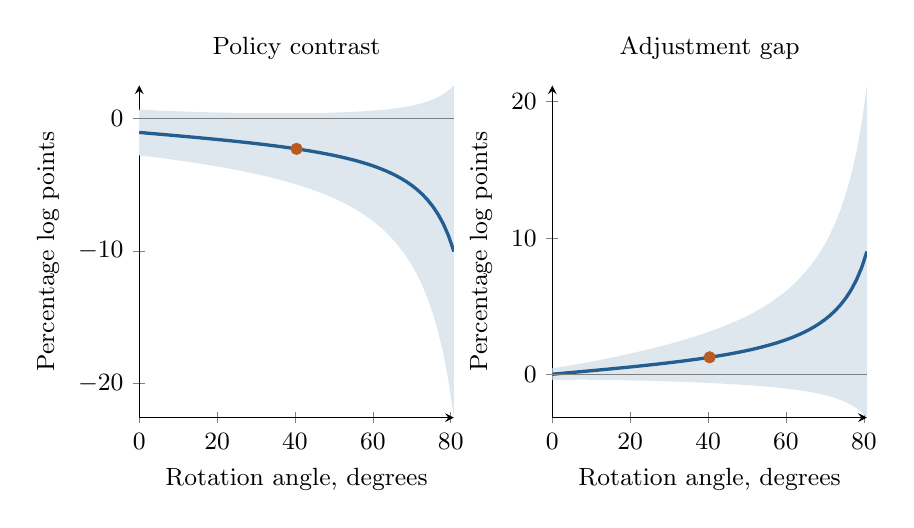
\begin{tikzpicture}
\begin{groupplot}[group style={group size=2 by 1,horizontal sep=1.25cm},
 width=.46\textwidth,height=5.8cm,axis lines=left,xmin=0,xmax=80.8,
 xtick={0,20,40,60,80},xlabel={Rotation angle, degrees},
 tick label style={font=\small},label style={font=\small},title style={font=\small},clip=true]
\nextgroupplot[title={Policy contrast},ylabel={Percentage log points}]
\addplot[name path=lo,draw=none,forget plot] coordinates {(0,-2.7858367) (1.3466608,-2.8328569) (2.6933216,-2.8810189) (4.0399824,-2.930356) (5.3866433,-2.980905) (6.7333041,-3.032707) (8.0799649,-3.0858073) (9.4266257,-3.1402556) (10.773287,-3.1961068) (12.119947,-3.2534205) (13.466608,-3.3122622) (14.813269,-3.3727032) (16.15993,-3.4348211) (17.506591,-3.4987007) (18.853251,-3.5644341) (20.199912,-3.6321215) (21.546573,-3.7018722) (22.893234,-3.7738048) (24.239895,-3.848049) (25.586555,-3.9247458) (26.933216,-4.0040493) (28.279877,-4.0861274) (29.626538,-4.1711642) (30.973199,-4.2593609) (32.31986,-4.3509383) (33.66652,-4.4461388) (35.013181,-4.5452292) (36.359842,-4.6485036) (37.706503,-4.7562868) (39.053164,-4.8689386) (40.399824,-4.9868583) (41.746485,-5.1104902) (43.093146,-5.2403298) (44.439807,-5.3769321) (45.786468,-5.5209195) (47.133129,-5.6729935) (48.479789,-5.8339467) (49.82645,-6.0046784) (51.173111,-6.1862129) (52.519772,-6.3797223) (53.866433,-6.5865535) (55.213093,-6.8082625) (56.559754,-7.0466562) (57.906415,-7.3038451) (59.253076,-7.5823099) (60.599737,-7.8849861) (61.946398,-8.2153734) (63.293058,-8.5776775) (64.639719,-8.9769983) (65.98638,-9.4195796) (67.333041,-9.9131502) (68.679702,-10.467392) (70.026362,-11.094597) (71.373023,-11.810616) (72.719684,-12.636239) (74.066345,-13.599286) (75.413006,-14.737851) (76.759666,-16.105528) (78.106327,-17.780185) (79.452988,-19.87946) (80.799649,-22.58987)};
\addplot[name path=hi,draw=none,forget plot] coordinates {(0,0.67855499) (1.3466608,0.65709709) (2.6933216,0.63670528) (4.0399824,0.61733667) (5.3866433,0.5989515) (6.7333041,0.58151304) (8.0799649,0.56498744) (9.4266257,0.54934366) (10.773287,0.53455337) (12.119947,0.52059087) (13.466608,0.50743305) (14.813269,0.4950593) (16.15993,0.48345152) (17.506591,0.47259406) (18.853251,0.46247374) (20.199912,0.45307983) (21.546573,0.44440411) (22.893234,0.43644088) (24.239895,0.42918701) (25.586555,0.42264207) (26.933216,0.41680841) (28.279877,0.41169125) (29.626538,0.40729892) (30.973199,0.403643) (32.31986,0.40073856) (33.66652,0.39860443) (35.013181,0.39726355) (36.359842,0.39674336) (37.706503,0.39707619) (39.053164,0.39829989) (40.399824,0.40045837) (41.746485,0.4036024) (43.093146,0.4077905) (44.439807,0.41308992) (45.786468,0.41957795) (47.133129,0.42734337) (48.479789,0.43648823) (49.82645,0.44713003) (51.173111,0.45940426) (52.519772,0.47346762) (53.866433,0.48950186) (55.213093,0.50771862) (56.559754,0.52836529) (57.906415,0.55173258) (59.253076,0.57816382) (60.599737,0.60806709) (61.946398,0.6419306) (63.293058,0.68034293) (64.639719,0.72401961) (65.98638,0.77383867) (67.333041,0.83088889) (68.679702,0.89653637) (70.026362,0.97251794) (71.373023,1.0610752) (72.719684,1.1651511) (74.066345,1.2886866) (75.413006,1.437081) (76.759666,1.6179336) (78.106327,1.8422898) (79.452988,2.1268402) (80.799649,2.498053)};
\addplot[policyblue!15,draw=none,forget plot] fill between[of=lo and hi];
\addplot[policyblue,very thick] coordinates {(0,-1.0536408) (1.3466608,-1.0878799) (2.6933216,-1.1221568) (4.0399824,-1.1565097) (5.3866433,-1.1909767) (6.7333041,-1.225597) (8.0799649,-1.2604099) (9.4266257,-1.295456) (10.773287,-1.3307767) (12.119947,-1.3664148) (13.466608,-1.4024146) (14.813269,-1.4388219) (16.15993,-1.4756848) (17.506591,-1.5130533) (18.853251,-1.5509802) (20.199912,-1.5895208) (21.546573,-1.628734) (22.893234,-1.668682) (24.239895,-1.709431) (25.586555,-1.7510519) (26.933216,-1.7936204) (28.279877,-1.8372181) (29.626538,-1.8819327) (30.973199,-1.927859) (32.31986,-1.9750999) (33.66652,-2.0237672) (35.013181,-2.0739828) (36.359842,-2.1258801) (37.706503,-2.1796053) (39.053164,-2.2353194) (40.399824,-2.2932) (41.746485,-2.3534439) (43.093146,-2.4162697) (44.439807,-2.4819211) (45.786468,-2.5506708) (47.133129,-2.6228251) (48.479789,-2.6987293) (49.82645,-2.7787742) (51.173111,-2.8634043) (52.519772,-2.9531273) (53.866433,-3.0485258) (55.213093,-3.1502719) (56.559754,-3.2591454) (57.906415,-3.3760562) (59.253076,-3.502073) (60.599737,-3.6384595) (61.946398,-3.7867214) (63.293058,-3.9486673) (64.639719,-4.1264893) (65.98638,-4.3228705) (67.333041,-4.5411306) (68.679702,-4.7854276) (70.026362,-5.0610396) (71.373023,-5.3747705) (72.719684,-5.735544) (74.066345,-6.1552996) (75.413006,-6.650385) (76.759666,-7.2437972) (78.106327,-7.9689475) (79.452988,-8.87631) (80.799649,-10.045909)};
\addplot[gray,thin,forget plot] coordinates {(0,0)(80.8,0)};
\addplot[newsorange,only marks,mark=*,mark size=2pt,forget plot] coordinates {(40.399824,-2.2932)};
\nextgroupplot[title={Adjustment gap},ylabel={Percentage log points}]
\addplot[name path=lo,draw=none,forget plot] coordinates {(0,-0.41364985) (1.3466608,-0.40177637) (2.6933216,-0.39316665) (4.0399824,-0.3873327) (5.3866433,-0.38384812) (6.7333041,-0.38235114) (8.0799649,-0.38254087) (9.4266257,-0.38417032) (10.773287,-0.38703849) (12.119947,-0.39098275) (13.466608,-0.39587214) (14.813269,-0.40160163) (16.15993,-0.40808749) (17.506591,-0.41526342) (18.853251,-0.42307759) (20.199912,-0.43149017) (21.546573,-0.44047147) (22.893234,-0.45000041) (24.239895,-0.46006341) (25.586555,-0.47065345) (26.933216,-0.48176941) (28.279877,-0.49341559) (29.626538,-0.50560137) (30.973199,-0.51834098) (32.31986,-0.53165341) (33.66652,-0.54556246) (35.013181,-0.56009682) (36.359842,-0.57529028) (37.706503,-0.59118206) (39.053164,-0.60781726) (40.399824,-0.62524733) (41.746485,-0.64353082) (43.093146,-0.66273415) (44.439807,-0.68293262) (45.786468,-0.70421164) (47.133129,-0.72666815) (48.479789,-0.75041243) (49.82645,-0.77557015) (51.173111,-0.80228504) (52.519772,-0.830722) (53.866433,-0.861071) (55.213093,-0.89355182) (56.559754,-0.92842007) (57.906415,-0.96597459) (59.253076,-1.0065669) (60.599737,-1.0506132) (61.946398,-1.0986098) (63.293058,-1.1511536) (64.639719,-1.2089682) (65.98638,-1.2729399) (67.333041,-1.3441657) (68.679702,-1.4240199) (70.026362,-1.5142478) (71.373023,-1.6170993) (72.719684,-1.735526) (74.066345,-1.8734771) (75.413006,-2.0363608) (76.759666,-2.2317851) (78.106327,-2.470804) (79.452988,-2.7701175) (80.799649,-3.1562025)};
\addplot[name path=hi,draw=none,forget plot] coordinates {(0,0.45718334) (1.3466608,0.51378799) (2.6933216,0.57373213) (4.0399824,0.63660384) (5.3866433,0.70205344) (6.7333041,0.76979692) (8.0799649,0.83961252) (9.4266257,0.91133412) (10.773287,0.98484372) (12.119947,1.0600642) (13.466608,1.1369531) (14.813269,1.2154973) (16.15993,1.2957089) (17.506591,1.3776219) (18.853251,1.4612898) (20.199912,1.5467837) (21.546573,1.6341913) (22.893234,1.7236162) (24.239895,1.8151772) (25.586555,1.909009) (26.933216,2.0052621) (28.279877,2.1041036) (29.626538,2.2057185) (30.973199,2.3103107) (32.31986,2.418105) (33.66652,2.5293487) (35.013181,2.6443143) (36.359842,2.7633023) (37.706503,2.8866445) (39.053164,3.0147078) (40.399824,3.1478991) (41.746485,3.2866704) (43.093146,3.4315253) (44.439807,3.5830266) (45.786468,3.741805) (47.133129,3.9085701) (48.479789,4.0841227) (49.82645,4.2693703) (51.173111,4.4653455) (52.519772,4.6732285) (53.866433,4.8943745) (55.213093,5.1303475) (56.559754,5.3829628) (57.906415,5.6543389) (59.253076,5.9469648) (60.599737,6.263784) (61.946398,6.6083044) (63.293058,6.98474) (64.639719,7.3981987) (65.98638,7.8549327) (67.333041,8.3626788) (68.679702,8.9311269) (70.026362,9.5725789) (71.373023,10.302892) (72.719684,11.142866) (74.066345,12.120328) (75.413006,13.273383) (76.759666,14.655631) (78.106327,16.344951) (79.452988,18.458989) (80.799649,21.184272)};
\addplot[policyblue!15,draw=none,forget plot] fill between[of=lo and hi];
\addplot[policyblue,very thick] coordinates {(0,0.021766745) (1.3466608,0.056005812) (2.6933216,0.090282743) (4.0399824,0.12463557) (5.3866433,0.15910266) (6.7333041,0.19372289) (8.0799649,0.22853582) (9.4266257,0.2635819) (10.773287,0.29890261) (12.119947,0.33454073) (13.466608,0.37054049) (14.813269,0.40694785) (16.15993,0.44381072) (17.506591,0.48117925) (18.853251,0.5191061) (20.199912,0.55764676) (21.546573,0.59685993) (22.893234,0.63680789) (24.239895,0.67755692) (25.586555,0.7191778) (26.933216,0.76174634) (28.279877,0.80534401) (29.626538,0.85005856) (30.973199,0.89598488) (32.31986,0.9432258) (33.66652,0.99189311) (35.013181,1.0421087) (36.359842,1.094006) (37.706503,1.1477312) (39.053164,1.2034453) (40.399824,1.2613259) (41.746485,1.3215698) (43.093146,1.3843956) (44.439807,1.450047) (45.786468,1.5187967) (47.133129,1.590951) (48.479789,1.6668552) (49.82645,1.7469001) (51.173111,1.8315303) (52.519772,1.9212533) (53.866433,2.0166517) (55.213093,2.1183978) (56.559754,2.2272713) (57.906415,2.3441822) (59.253076,2.4701989) (60.599737,2.6065854) (61.946398,2.7548473) (63.293058,2.9167932) (64.639719,3.0946152) (65.98638,3.2909964) (67.333041,3.5092566) (68.679702,3.7535535) (70.026362,4.0291655) (71.373023,4.3428964) (72.719684,4.7036699) (74.066345,5.1234255) (75.413006,5.6185109) (76.759666,6.2119231) (78.106327,6.9370734) (79.452988,7.8444359) (80.799649,9.0140345)};
\addplot[gray,thin,forget plot] coordinates {(0,0)(80.8,0)};
\addplot[newsorange,only marks,mark=*,mark size=2pt,forget plot] coordinates {(40.399824,1.2613259)};
\end{groupplot}
\end{tikzpicture}
\caption{Complete admissible rotation assessment. Curves are twelve-month point projections per ten-basis-point rate-factor contribution; orange points identify the author median. Shading projects one joint 95 per cent ellipsoid and simultaneously covers the retained-factor family under its regularity assumptions. The curves include continuous closure limits, not a fitted singular zero-angle model. Factor and sign-boundary estimation uncertainty is not covered.}
\label{fig:rotation}
\end{figure}
% END ROTATION_FIGURE

The closure point bounds are $[-10.05,-1.05]$ for the policy contrast and $[0.02,9.01]$ for the gap; both strict-sign endpoints are excluded. Their directions persist in this family, but their magnitudes are highly dependent on the rotation. A single joint 95 per cent ellipsoid for $(b_r,b_v,\gamma)$ gives simultaneous conditional envelopes $[-22.59,2.50]$ and $[-3.16,21.18]$, respectively. These cover every retained-factor angle under the joint score assumptions; a collection of unrelated pointwise intervals would not provide this guarantee. They condition on the supplied factor, event QR and sign-set endpoints, leaving their estimation uncertainty uncovered. The lower endpoint has a zero information-rate normalisation and is not fitted: I report continuous limits of the defined policy and gap contrasts. The information coefficient diverges there. At the upper boundary its equity loading is zero, also excluded by the strict signs. A primitive-coordinate Bonferroni companion also covers the continuum under marginal regularity, without requiring an invertible joint covariance: its gap envelope is $[-1.31,20.06]$.

Financial signs do not verify exogeneity. The supplementary zero-product test fails to reject close to the lower boundary.

\subsection{A causal direction and falsification checks}

For a latent policy innovation contributing ten basis points to the same factor, let its measured direction be $(1-a,a)^\top$. Under the constant noiseless mapping, invariant response and orthogonality assumptions in Appendix~\ref{app:causal-bridge}, its relative response and adjustment are
\begin{equation}
 \tau(a)=(1-a)\beta_m+a\beta_c,
 \qquad \gamma-\tau(a)=(w-a)\theta.
 \label{eq:causal-direction}
\end{equation}
At $a=0$ the projection gap equals the causal adjustment; when $\theta\ne0$, this equality requires $a=0$. This coordinate is not an estimated contamination probability; without restrictions it may lie outside $[0,1]$. The illustrative range $a\in[0,1]$ imposes non-negative measured loadings; it is a sensitivity assumption, distinct from the financial rotation restrictions. At the median projection, the response point is $-2.29$ at $a=0$, $-1.56$ at $a=0.25$ and $-0.82$ at $a=0.50$. Its sign changes at $a=0.777$, while the adjustment changes sign already at $a=w=0.427$. A common 95 per cent coefficient ellipse gives an upper response bound $0.07$ even at $a=0$, so the individual policy interval's exclusion of zero is not simultaneous separation evidence. An imposed absolute outcome-bias bound $B$ widens each response envelope by $B$ on either side; neither $a$ nor $B$ is identified here.

I also regress three predetermined production changes, measured from $t-26$ to $t-13$, on the primary components and controls. They precede the controlled twelve-month growth history and cannot be caused by the current announcement. Joint two-component tests give $p=0.674$, $0.714$ and $0.827$ for durables, non-durables and their difference; Bonferroni adjustment across the family yields no rejection. The contrast's policy coefficient is $0.63$ with standard error $1.10$. These imprecise retrospective checks do not reconstruct real-time public information or verify exclusion. Serially predictable news, omitted public-news responses and measurement error remain possible.

LP-IV can identify a policy response with a relevant, excluded proxy and an explicit normalisation \citep[\S\S1.3--1.5, 2]{StockWatson2018}. Reusing a supplied component as its own instrument verifies none of those conditions. The retained data contain no independently justified excluded proxy or public-news forecast-surprise measure. I therefore report the conditional response and its sensitivity rather than claim an unconditional causal effect.

\section{Economic interpretation and limitations}
\label{sec:interpretation}

Both groups have negative primary policy point responses, with durables more negative. This is compatible with user-cost amplification, but production and nominal factor units do not identify a household elasticity. The response ranking and residualised mixture explain the positive point adjustment without requiring relative information-induced expansion. The extension locates an additional limitation: the retained estimates preserve this point direction within the sign-admissible family while permitting large magnitude variation. A directionally stable set of point estimates is weaker evidence than a sampling envelope excluding zero.

In Germany, orthogonality excludes announcement-correlated energy, foreign-demand or supply news with unequal sector effects. Differencing removes only identical loadings. Public-news policy responses can also covary with the remaining production disturbance despite conventional financial signs \citep{BauerSwanson2023a}. Controlling the information-labelled contribution does not prove the policy-labelled contribution exogenous. The retained window, restrictions and predetermined-outcome checks cannot verify these exclusions.

Inventory, export demand, financing and postponed purchases are possible mechanisms, not separately identified channels. The contrast is neither household expenditure, a motor-vehicle response nor a physical production share. Converting its factor normalisation into an actual policy-rate intervention requires an additional identification and scaling argument.

The sample spans unconventional policy, tightening and pandemic states. Joint period tests are imprecise and common-dynamics restrictions do not establish structural invariance. Revised controls are not the real-time information set. Independent numerical agreement validates implementation; it does not validate exogeneity, response stability or the factor's construction. Confidence statements remain asymptotic and conditional on the retained source.

\section{Conclusion}
\label{sec:conclusion}

Separating current policy news makes the median durable-minus-non-durable production point response more negative, giving a $1.26$ adjustment. Its locked conservative interval includes zero. Joint construction and period contrasts also do not establish tight equivalence. The entire admissible rotation family preserves a positive point adjustment but permits a range of $0.02$--$9.01$, with a common conditional sampling envelope including zero. The supplementary rejection for the median construction consequently cannot establish a precise, construction-invariant result.

The stock-flow benchmark explains why purchases can be sensitive to financing and demand news, while production aggregates several channels. The latent-direction calculation shows exactly when the projection adjustment can be interpreted causally and how that conclusion changes with imperfect separation. Predetermined-outcome non-rejection does not close the identifying assumptions. The contribution is a checked assessment of measurement, uncertainty and economic interpretation in a defined German contrast; an unconditional causal policy effect remains unidentified by the retained evidence.

\setcounter{mainsections}{\value{section}}
\appendix
\setcounter{equation}{0}
\renewcommand{\theequation}{A.\arabic{equation}}
\renewcommand{\theHequation}{A.\arabic{equation}}
\section{Projection identities and uncertainty}
\label{app:projection}

I apply the established partial-regression and covariance results of \citet[Sections 2--3 and Appendix A]{Ding2021}. The supplied factor is fixed; regressors and their population projection weights remain random.

\subsection{The exact sample comparison}
\label{app:sample}

Fix a horizon and suppress its subscript. Let $Y,m,c\in\mathbb R^n$ refer to identical observations, with $r=m+c$ in common units. The $n\times q$ control matrix $Z$ includes an intercept. I require $\operatorname{rank}(Z)=q$, $\operatorname{rank}[Z,m,c]=q+2$ and $n>q+2$. Define
\begin{align}
 M_Z&=I-Z(Z^\top Z)^{-1}Z^\top,
 & y&=M_ZY,\notag\\
 a&=M_Zm,
 & b&=M_Zc,\qquad s=a+b.\label{eq:app-residualise}
\end{align}
Thus $M_Z^\top=M_Z$, $M_Z^2=M_Z$ and $M_ZZ=0$. The residualised matrix $A=[a,b]$ has rank two, so $A^\top A$ is positive definite and $s^\top s>0$.

\begin{proof}[Proof of Proposition~\ref{prop:mixture}]
Profiling the nuisance coefficient gives $\widehat\eta(\beta)=(Z^\top Z)^{-1}Z^\top(Y-m\beta_m-c\beta_c)$ and criterion $\|y-A\beta\|^2$. Hence $\widehat\beta=(A^\top A)^{-1}A^\top y$, and $\widehat e=y-A\widehat\beta$ is orthogonal to both $a$ and $b$. The reduced normal equation gives
\begin{equation}
 \widehat\gamma=\frac{s^\top y}{s^\top s}
 =\frac{s^\top a}{s^\top s}\widehat\beta_m
  +\frac{s^\top b}{s^\top s}\widehat\beta_c,
 \quad s^\top a+s^\top b=s^\top s.
 \label{eq:app-normal-equations}
\end{equation}
Subtracting $\widehat\beta_m$ proves \eqref{eq:sample-gap}.
\end{proof}

This is an identity for every $Y$, without probabilistic assumptions. It does not survive different rows, controls, scaling or a different definition of $r$. Expanding its weight shows why it need not be a probability or variance share:
\begin{align}
 \widehat w_c
 &=\frac{b^\top b+a^\top b}{a^\top a+b^\top b+2a^\top b}.\label{eq:app-nonconvex}
\end{align}
Negative weights or weights above one are possible. If $\widehat w_c=0$, the sample gap is zero for every outcome although $\widehat\theta$ need not vanish. Event-level orthogonality also does not imply controlled monthly orthogonality: for an aggregation matrix $H$, the relevant inner product is $m_e^\top H^\top M_ZHc_e$, rather than $m_e^\top c_e$.



\subsection{Population weights and their influence}
\label{app:population}

Let the corresponding population projections exist with nonsingular moment matrices. Expectations below use the stable population moments, or their periodically structured limits, required by the design. A tilde denotes population linear residualisation on $Z$. Write $\widetilde r=r-Z^\top\pi_r$ and $\widetilde c=c-Z^\top\pi_c$, where $\mathbb E[Z\widetilde r]=\mathbb E[Z\widetilde c]=0$. Put
\begin{align}
 B&=\mathbb E[\widetilde r^2]>0,
 & C&=\mathbb E[\widetilde r\widetilde c],
 & w_c&=C/B, &\theta&=\beta_c-\beta_m.\label{eq:app-population-weight}
\end{align}
For the full residual $e$, the projection normal equations give $\mathbb E[Ze]=\mathbb E[me]=\mathbb E[ce]=0$. Therefore $\gamma=B^{-1}\mathbb E[\widetilde r\widetilde Y]=\beta_m+w_c\theta$. The reduced residual consequently differs from the full residual:
\begin{align}
 \widetilde Y&=\beta_m\widetilde r+\theta\widetilde c+e,
 & v&=e+\theta(\widetilde c-w_c\widetilde r).\label{eq:app-reduced-residual}
\end{align}

The nuisance projections do not add first-order terms to $C$ or $B$, because
\begin{align}
 \partial_{\pi_r}C&=-\mathbb E[Z\widetilde c]=0,
 &\partial_{\pi_c}C&=-\mathbb E[Z\widetilde r]=0,
 &\partial_{\pi_r}B&=-2\mathbb E[Z\widetilde r]=0.\label{eq:app-nuisance}
\end{align}
Thus, under regular asymptotic linearity, their moment influences are $\widetilde r_t\widetilde c_t-C$ and $\widetilde r_t^2-B$. Differentiating their ratio gives
\begin{align}
 \psi_{w,t}
 &=\frac{(\widetilde r_t\widetilde c_t-C)-w_c(\widetilde r_t^2-B)}{B}
  =\frac{\widetilde r_t(\widetilde c_t-w_c\widetilde r_t)}{B}.\label{eq:app-weight-influence}
\end{align}

For $\xi_t=(\widetilde m_t,\widetilde c_t)^\top$ and $Q=\mathbb E[\xi_t\xi_t^\top]$, the full coefficient influence is $\psi_{\beta,t}=Q^{-1}\xi_t e_t$, while $\psi_{\gamma,t}=\widetilde r_t v_t/B$. Define $\psi_{\theta,t}=(-1,1)\psi_{\beta,t}$. The row identity $(1-w_c,w_c)=\mathbb E[\widetilde r\xi^\top]/B$ implies
\begin{align}
 \frac{\widetilde r_t e_t}{B}
  &=(1-w_c,w_c)\psi_{\beta,t}
    =\psi_{\beta_m,t}+w_c\psi_{\theta,t},\\
 \psi_{\delta,t}
  &=\psi_{\gamma,t}-\psi_{\beta_m,t}
    =w_c\psi_{\theta,t}+\theta\psi_{w,t}.\label{eq:app-gap-influence}
\end{align}
Hence the long-run variance contains
\begin{align}
 \mathcal V_\delta
 &=w_c^2\mathcal V_\theta+\theta^2\mathcal V_w
   +2w_c\theta\mathcal C_{\theta,w},\label{eq:app-gap-variance}
\end{align}
Here $\mathcal C_{\theta,w}$ is the long-run covariance. Under a genuinely fixed design $\mathcal X$, the sample identity gives $\Var(\widehat\delta\mid\mathcal X)=\widehat w_c^2\Var(\widehat\theta\mid\mathcal X)$; marginal HAC need not estimate this conditional variance. If $w_c=0\ne\theta$, weight variation leads; if $\theta=0\ne w_c$, response-difference variation leads. At the double zero the product gradient vanishes. These distinct null geometries motivate coordinate-set inference.

\subsection{Joint covariance and conservative product bounds}
\label{app:covariance}

I fit the full, reduced and weight regressions, respectively, with $X_F=[m,c,Z]$, $X_R=[r,Z]$ and $X_W=X_R$, using responses $Y,Y,c$ and each regression's own residual $\widehat u_{j,t}$. Let $\ell_{j,t}$ be column $t$ of $L_j=(X_j^\top X_j)^{-1}X_j^\top$. The distinction between the population-scale influence and the numerical coefficient contribution is
\begin{align}
 \widehat\psi_{j,t}
 &=\widehat Q_j^{-1}x_{j,t}\widehat u_{j,t}
   =n\ell_{j,t}\widehat u_{j,t},
 &\widehat Q_j&=X_j^\top X_j/n,
 &a_{j,t}&=\widehat\psi_{j,t}/n.\label{eq:app-contribution}
\end{align}
I compute $L_j$ through the full-rank QR factorisation. Let $a_t$ collect the contributions for $\beta_m$, $\beta_c$, $\gamma$ and $w_c$. It satisfies $a_{\delta,t}=a_{\gamma,t}-a_{\beta_m,t}=\widehat w_c a_{\theta,t}+\widehat\theta a_{w,t}$. Its four-dimensional first-order covariance is therefore generally singular; no rank-four inversion is required.

For origin-month ordinals $\tau_i$, the calendar Bartlett covariance is
\begin{align}
 \widehat V
 &=\kappa\sum_{i=1}^n\sum_{j=1}^n
       K_{L_h}(|\tau_i-\tau_j|)a_i a_j^\top,
 &\kappa&=\frac{n}{n-k_F},\qquad k_F=q+2,\label{eq:app-hac}\\
 K_L(d)&=\max\{1-d/(L+1),0\},
 &L_h&=h+\left\lceil4(n/100)^{2/9}\right\rceil.\label{eq:app-kernel}
\end{align}
Equivalently, the summands are $\widehat\psi_i\widehat\psi_j^\top/n^2$. Calendar gaps, cross-model blocks and the common correction are retained. Consistency still requires the score limit and moment conditions in Section~\ref{sec:uncertainty}; the finite-sample multiplier does not give exact coverage.

A fixed linear transformation of $\widehat V$ yields the covariance of $(\widehat\beta_m,\widehat\delta,\widehat w_c,\widehat\theta)$, retaining its cross-model blocks. Likewise, shared sector regressions obey $\widehat\beta_m=\widehat\beta_{D,m}-\widehat\beta_{N,m}$ and
\begin{align}
 \widehat{\operatorname{Var}}(\widehat\beta_m)
 &=\widehat V_{D,m}+\widehat V_{N,m}
       -2\widehat{\operatorname{Cov}}(\widehat\beta_{D,m},\widehat\beta_{N,m}).\label{eq:app-sector-covariance}
\end{align}
This covariance cannot be inferred from separate significance labels.

\begin{proposition}[Conservative product interval]
\label{prop:app-product}
Suppose $I_w=[w_-,w_+]$ and $I_\theta=[\theta_-,\theta_+]$ each cover their population coordinate with asymptotic probability at least $1-\alpha/2$. Then
\begin{align}
 I_\delta&=\left[
 \min_{s,t\in\{-,+\}}w_s\theta_t,
 \max_{s,t\in\{-,+\}}w_s\theta_t\right]\label{eq:app-product-bounds}
\end{align}
has asymptotic coverage at least $1-\alpha$ for $\delta=w_c\theta$.
\end{proposition}
\begin{proof}
Separate linearity places the product extrema at rectangle corners. The union bound gives $\Pr\{\delta\in I_\delta\}\ge1-\Pr\{w_c\notin I_w\}-\Pr\{\theta\notin I_\theta\}$. Taking the lower limit proves the result without independence or an invertible covariance.
\end{proof}

At $\alpha=0.05$, the normal critical value $z_{1-\alpha/4}$ gives 97.5 per cent coordinate intervals. I do not clip weights. Even at the double zero, coverage follows if both coordinates have valid nondegenerate marginal inference; it does not cure marginal degeneracy or cover the supplied factor's construction.

\setcounter{table}{0}
\renewcommand{\thetable}{B.\arabic{table}}
\renewcommand{\theHtable}{B.\arabic{table}}

\section{Source reconciliation}
\label{app:source_reconciliation}

Table~\ref{tab:source_coverage} distinguishes source coverage from the estimation samples. I retain the 15 September snapshot unchanged alongside the active 10 October snapshot. The production update adds August 2026 and revises July non-durable production from 92.3 to 91.4; other overlapping production observations and the historical HICP request are unchanged. The author-supplied shock CSVs are unchanged between these retrievals.

\begin{table}[htbp]
\centering
\caption{Coverage of retained source observations}
\label{tab:source_coverage}
\begin{tabular}{@{}lccr@{}}
\toprule
Source & First & Last & Observations \\
\midrule
Production, each grouping & 1991-01 & 2026-08 & 428 \\
Historical all-items HICP & 1996-01 & 2025-12 & 360 \\
Monthly contributions & 1999-01 & 2025-10 & 322 \\
Event contributions & 1999-01-07 & 2025-10-30 & 312 \\
\bottomrule
\end{tabular}
\end{table}

The EA-MPD workbook contains 315 dated rows. The update explicitly excludes 13 September 2001, 17 September 2001 and 8 October 2008, leaving exactly 312 retained events. Its code records a joint Fed--ECB US-dollar swap announcement, a joint cut at 17:30 and a joint cut, respectively. There are 277 months with retained events and 45 without. Six event factors are observed zeros with nonzero equity surprises and offsetting nonzero median contributions; they differ from empty-event months. No retained four-maturity rate or equity input is missing after these exclusions. All six monthly fields equal event sums to retained numerical precision, and the uncentred component and median rotation reproduce the supplied eight-decimal values. Exact source URLs, the pinned revision and checksums are retained with the data manifest.
\subsection{Specification record and numerical replay}
\label{app:record}

I recorded the primary specification at 21:30 UTC on 10 October 2026 and committed revision \texttt{66ed69c} before the first response execution at 23:07 UTC. Its outcome, horizon, sample, components, controls and interval remain unchanged. The economic benchmark, measurement bridge and supplementary zero-product assessment were later additions. The joint stability, full-rotation and causal-sensitivity extension was recorded at 15:09 UTC on 11 October, after all original results and source-only rotation algebra were known but before its new outcome contrasts and diagnostics. It adds the declared fits in Section~\ref{sec:extension}; it is an informed extension, not blind registration or a revised primary hypothesis.

The six-lag and poor-man comparisons retain the primary origins. The earlier-period check requires $t+h\le\text{December 2019}$, so its twelve-month origins end in December 2018. The short and long bandwidths are $h+\lceil B/2\rceil$ and $h+2B$, respectively, for $B=\lceil4(n/100)^{2/9}\rceil$. These were declared sensitivities, rather than departures selected from the results. Table~\ref{tab:sensitivities} records the numerical comparisons.

% BEGIN SENSITIVITY_TABLE
\begin{table}[htbp]
\centering\small
\caption{Numerical sensitivity comparisons at twelve months}
\label{tab:sensitivities}
\begin{tabular}{@{}lrrrrr@{}}
\toprule
Specification & $n$ & $\widehat\beta_m$ & Normal 95\% interval & $\widehat\delta$ & Product 95\% bounds \\
\midrule
Primary & 308 & $-2.29$ & $[-4.18,-0.40]$ & $1.26$ & $[-0.11,3.31]$ \\
Six lags, matched & 308 & $-2.52$ & $[-4.62,-0.42]$ & $1.17$ & $[-0.16,3.13]$ \\
Poor-man components & 308 & $-2.27$ & $[-4.06,-0.47]$ & $1.23$ & $[-1.02,4.19]$ \\
Pre-pandemic endpoints & 228 & $-2.08$ & $[-4.28,0.11]$ & $0.66$ & $[-1.44,3.09]$ \\
Short bandwidth & 308 & $-2.29$ & $[-4.16,-0.43]$ & $1.26$ & $[-0.08,3.27]$ \\
Long bandwidth & 308 & $-2.29$ & $[-4.25,-0.34]$ & $1.26$ & $[-0.14,3.36]$ \\
\bottomrule
\end{tabular}
\par\smallskip\begin{minipage}{.97\textwidth}\footnotesize
All responses use the same ten-basis-point factor units. Six-lag and poor-man comparisons retain the primary origins. Pre-pandemic endpoints end by December 2019. Short and long bandwidths are 15 and 24, versus 18 in the primary regression, leaving its coefficients unchanged. Intervals are pointwise and retain the declared primary uncertainty target.
\end{minipage}
\end{table}
% END SENSITIVITY_TABLE

An independent base-R reconstruction checks transformations, controls, samples, QR coefficients, joint calendar covariance and intervals for nine cases. Its 351 comparisons agree within approximately $1.04\times10^{-13}$. This verifies calculation on the same inputs, not independent empirical replication. The \href{https://github.com/Amanjeet-S/Monetary-Policy}{private research repository} retains data, code, results and the consulted-source register; copyrighted article texts and the ECB workbook remain separately stored.
\setcounter{equation}{0}
\renewcommand{\theequation}{C.\arabic{equation}}
\renewcommand{\theHequation}{C.\arabic{equation}}
\section{Economic mechanism and causal measurement}
\label{app:economic-derivations}

\subsection{Durable services, user cost and purchase adjustment}
\label{app:household}

I derive a partial household benchmark using the established stock-service distinction of \citet[pp.~418--420]{Mankiw1982} and \citet[pp.~985--986, 990--992]{BarskyEtAl2007}; it is not a new durability theorem. Let $0<\alpha<1$, $0<\beta_H<1$, $0<d\le1$, $p_t>0$ and $\rho_t>-1$. Consumption and stock are positive; purchases and bond holdings are interior, resale is allowed, and feasibility and transversality hold. There are no adjustment costs. With the stock law \eqref{eq:stock-law}, the household chooses consumption, stock and a bond with next-period face-value payoff $B_t$ to maximise
\begin{align}
 \max_{\{C_t,S_t,B_t\}}\quad
 &\E_0\sum_{t\ge0}\beta_H^t\{\alpha\log C_t+(1-\alpha)\log S_t\},\notag\\
 \text{subject to}\quad
 &C_t+p_tX_t+\frac{B_t}{1+\rho_t}=W_t+B_{t-1},\quad t\ge0.
 \label{eq:household-problem}
\end{align}
Resources $W_t$ are in non-durable units. The real risk-free return $\rho_t$, depreciation and discount factor refer to the same period. This return differs from the nominal recomposed announcement factor $r_t$.

Let $\lambda_t=\alpha/C_t$. Varying the bond and end-of-period stock gives
\begin{align}
 \frac{\lambda_t}{1+\rho_t}&=\beta_H\E_t\lambda_{t+1},\label{eq:bond-euler}\\
 \lambda_tp_t&=\frac{1-\alpha}{S_t}
      +\beta_H(1-d)\E_t[\lambda_{t+1}p_{t+1}].\label{eq:stock-euler}
\end{align}
The stock condition values current services and the retained stock's next-period resale value. Set $M_{t+1}=\beta_H\lambda_{t+1}/\lambda_t$. Dividing \eqref{eq:stock-euler} by $\lambda_t$ proves \eqref{eq:user-cost}, including positive $q_t$. The bond condition and covariance decomposition then imply
\begin{equation}
 q_t=p_t-\frac{1-d}{1+\rho_t}\E_tp_{t+1}
             -(1-d)\Cov_t(M_{t+1},p_{t+1}).
 \label{eq:risky-user-cost}
\end{equation}
A negative covariance raises user cost relative to the expectation-only expression: resale is less valuable in high-marginal-utility states. Both this risk term and expected prices can change with announcement news.\footnote{This household valuation covariance differs from the observed announcement-time rate--equity covariance; it is not estimated by the production regressions.}

Under certainty and constant relative prices, $q_t=p(\rho_t+d)/(1+\rho_t)$, requiring $\rho_t+d>0$. This simplification does not require stationary consumption. Stationary consumption at a benchmark would additionally require $\beta_H(1+\bar\rho)=1$.

\begin{samepage}
At a stationary-stock base, $\bar X=d\bar S>0$. Holding inherited stock fixed gives $\mathrm dX_t=\mathrm dS_t$ and hence
\begin{align}
 \mathrm d\log X_t&=\frac1d\mathrm d\log S_t
   =\frac1d(\mathrm d\log C_t-\mathrm d\log q_t),\label{eq:flow-proof}\\
 \left.\frac{\partial\log X_t}{\partial\rho_t}\right|_{C_t,S_{t-1},p}
   &=-\frac{1-d}{d(1+\rho_t)(\rho_t+d)}.\label{eq:rate-flow-derivative}
\end{align}
\end{samepage}
Subtracting $\mathrm d\log C_t$ proves \eqref{eq:relative-flow}. The rate derivative is negative at $d<1$ and zero at $d=1$, locally holding inherited stock and current consumption fixed. It is not a steady-state comparison. Zero depreciation, no-resale corners, adjustment costs and endogenous consumption or prices can invalidate the interpretation. The positive-purchase neighbourhood, with current $C_t$ fixed, is
\begin{equation}
 X_t(q_t)=\bar S\{\bar q/q_t-(1-d)\}>0
 \quad\Longleftrightarrow\quad q_t<\bar q/(1-d),\quad 0<d<1.
 \label{eq:purchase-neighbourhood}
\end{equation}
As $d\to0$, amplification grows but this contraction neighbourhood shrinks; the local derivative does not imply a large finite elasticity.

\subsection{A conditional bridge from components to causal responses}
\label{app:causal-bridge}

For a fixed horizon, suppose a stable linear structural relation and a noiseless measurement equation hold:
\begin{equation}
 Y_{t,h}=b_h^\top\varepsilon_t+Z_t^\top\eta_h+\nu_{t,h},
 \qquad s_t=A\varepsilon_t.
 \label{eq:structural-measurement}
\end{equation}
The constant $A$ is invertible and $Q_s=\E[\widetilde s_t\widetilde s_t^\top]$ is positive definite. Tildes denote population linear residualisation on the same $Z_t$. Maintain $\E[\widetilde s_t\nu_{t,h}]=0$, which implies orthogonality to the residualised disturbance. Since $\widetilde\varepsilon_t=A^{-1}\widetilde s_t$,
\begin{equation}
 \beta_h=Q_s^{-1}\E[\widetilde s_t\widetilde Y_{t,h}]
        =Q_s^{-1}Q_sA^{-\top}b_h=A^{-\top}b_h.
 \label{eq:bridge-proof}
\end{equation}
A known ordered diagonal mapping gives $b_{m,h}=a_m\beta_{m,h}$ and $b_{c,h}=a_c\beta_{c,h}$. A known dense mapping instead recovers responses jointly through $b_h=A^\top\beta_h$; each latent column must be checked to interpret a supplied coefficient separately. Unknown mixing, measurement noise or non-orthogonal production disturbances can invalidate the causal reading. Observed-column orthogonality does not establish these restrictions. Here $b_h$ is a difference of sector responses, not an intervention on a physical production ratio.


\setcounter{equation}{0}
\renewcommand{\theequation}{D.\arabic{equation}}
\renewcommand{\theHequation}{D.\arabic{equation}}
\setcounter{table}{0}
\renewcommand{\thetable}{D.\arabic{table}}
\renewcommand{\theHtable}{D.\arabic{table}}
\section{Supplementary zero-product inference}
\label{app:gap-tests}

The null is $H_0=H_w\cup H_\theta$, where the coordinate nulls are $w=0$ and $\theta=0$. Let $p_w,p_\theta$ be the existing two-sided normal marginal $p$-values, asymptotically valid under their respective nulls. The established intersection-union principle \citep[\S3, Theorem~1]{BergerHsu1996} gives
\begin{equation}
 p_{\mathrm{IUT}}=\max\{p_w,p_\theta\}.\label{eq:iut-p}
\end{equation}
At any parameter point $a\in H_0$, at least one coordinate null $H_j$ is true, so
\begin{equation}
 \limsup_n\Pr_a(p_{\mathrm{IUT}}\le\alpha)
 \le\limsup_n\Pr_a(p_j\le\alpha)\le\alpha.\label{eq:iut-size}
\end{equation}
No independence is required; the level is pointwise asymptotic, not finite-sample or uniform. Primary rectangle rejection requires both marginal $p$-values below $0.025$ and is nested within the supplementary 5 per cent gate. This nesting does not justify broader post-estimation selection.

For $a=(w,\theta)^\top$, maintain a nondegenerate joint limit and consistent coefficient covariance:
\begin{equation}
 \sqrt n(\widehat a-a)\overset{d}{\longrightarrow}N(0,\Omega_a),\qquad
 n\widehat V_a\overset{p}{\longrightarrow}\Omega_a\succ0.
 \label{eq:ellipse-limit}
\end{equation}
With positive-definite $\widehat V_a$, the first-order 95 per cent joint region and its product image are
\begin{align}
 \mathcal E_{.95}&=\{a:(a-\widehat a)^\top\widehat V_a^{-1}(a-\widehat a)
                 \le\chi^2_{2,.95}\},\label{eq:joint-ellipse}\\
 I_{\delta,\mathcal E}&=\left[\min_{a\in\mathcal E_{.95}}w\theta,
                         \max_{a\in\mathcal E_{.95}}w\theta\right].\label{eq:ellipse-product}
\end{align}
Joint coordinate coverage implies product coverage. Let $\widehat V_a=LL^\top$ be the lower-triangular Cholesky factorisation and $k=\sqrt{\chi^2_{2,.95}}$. Define $\ell_1=kL_{11}$, $\ell_2=kL_{21}$ and $\ell_3=kL_{22}$, with $\ell_1,\ell_3>0$. The boundary is
\begin{equation}
 w(\phi)=\widehat w+\ell_1\cos\phi,\qquad
 \theta(\phi)=\widehat\theta+\ell_2\cos\phi+\ell_3\sin\phi.
 \label{eq:ellipse-boundary}
\end{equation}
The boundary product is quadratic in the sine and cosine coordinates. Its extrema are a two-dimensional instance of the confidence-set optimisation in Appendix~\ref{app:extension}, with $H_{12}=H_{21}=1/2$. The primary implementation independently solves the stationary half-angle polynomial, retaining all real roots, reduced-degree cases and the omitted angle $\phi=\pi$. The only interior stationary point of $w\theta$ is the origin, a saddle. Independent optimisation checks the global extrema. This projects coordinate uncertainty rather than imposing a regular product gradient.

The zero-product set is the union of the coordinate axes. Profiling the quadratic distance over each axis gives
\begin{equation}
 0\in I_{\delta,\mathcal E}\quad\Longleftrightarrow\quad
 \min\left\{\frac{\widehat w^2}{\widehat V_{ww}},
            \frac{\widehat\theta^2}{\widehat V_{\theta\theta}}\right\}
 \le\chi^2_{2,.95}.\label{eq:ellipse-zero}
\end{equation}
The primary response-difference statistic squared is approximately $4.41$, below the ellipse threshold $5.99$, explaining its inclusion of zero. These procedures summarise the same gap without repairing inaccurate score inference, construction uncertainty or announcement endogeneity.

% BEGIN FOLLOWUP_TABLE
\begin{table}[htbp]
\centering\small
\caption{Post-estimation twelve-month zero-gap assessment}
\label{tab:gap-followup}
\begin{tabular}{@{}lrl@{}}
\toprule
Specification & Intersection-union $p$ & Joint-ellipse product 95\% bounds \\
\midrule
Primary & $0.036$ & $[-0.19,3.18]$ \\
Six lags & $0.043$ & $[-0.24,2.82]$ \\
Poor-man components & $0.174$ & $[-1.17,3.03]$ \\
Pre-pandemic endpoints & $0.414$ & $[-1.25,2.94]$ \\
Short bandwidth & $0.033$ & $[-0.17,3.12]$ \\
Long bandwidth & $0.039$ & $[-0.21,3.26]$ \\
\bottomrule
\end{tabular}
\par\smallskip\begin{minipage}{.97\textwidth}\footnotesize
The same six designs and ten-basis-point factor units are retained. Nominal levels require valid marginal or joint asymptotic inference. The procedures were recorded after primary inspection and preliminary diagnostic arithmetic; they do not replace the primary product bounds. No confidence claim across all six designs is made.
\end{minipage}
\end{table}
% END FOLLOWUP_TABLE

The August 2026 production endpoint limits twelve-month origins to August 2025. Existing shocks reach October 2025; the next two origins require later production endpoints. Revisions or additional announcement dates do not create independent realised outcomes for the defined German contrast.

\setcounter{equation}{0}
\renewcommand{\theequation}{E.\arabic{equation}}
\renewcommand{\theHequation}{E.\arabic{equation}}
\section{Joint stability, rotation and causal sensitivity}
\label{app:extension}

For two fitted designs, let $a_{j,t}$ collect the weight and response-difference coefficient contributions, with zeros outside its origin sample. Put $g_t=(\sqrt{\kappa_1}a_{1,t}^\top,\sqrt{\kappa_2}a_{2,t}^\top)^\top$, $\kappa_j=n_j/(n_j-k_j)$. A common calendar kernel gives
\begin{equation}
 \widehat V_q=\sum_{t,s}K_L(|t-s|)g_tg_s^\top,
 \qquad q=(w_1,\theta_1,w_2,\theta_2)^\top.
 \label{eq:joint-stability-covariance}
\end{equation}
This retains overlapping-sample and cross-model covariance. For asymptotic inference I require sample fractions with positive limits, fixed dimensions, a joint Gaussian coordinate limit and consistent common-kernel covariance under the appropriate period-specific moments, $\sqrt n(\widehat q-q)\Rightarrow N(0,\Omega_q)$ and $n\widehat V_q\to_p\Omega_q\succ0$, with $n$ the full origin count. Padding absent contributions does not establish these conditions; arbitrary breaks can invalidate the approximation.

Define symmetric $H$ with $H_{12}=H_{21}=-1/2$, $H_{34}=H_{43}=1/2$ and other entries zero. The difference is $q^\top Hq$. If $CC^\top=\chi^2_{4,.95}\widehat V_q$, its image is the extrema over $\|u\|\le1$ of
\begin{equation}
 \widehat q^\top H\widehat q+2u^\top C^\top H\widehat q+u^\top C^\top HCu.
 \label{eq:quadratic-stability-image}
\end{equation}
For minimisation write this as $d+b^\top u+u^\top Gu$. The global solution satisfies $(G+\lambda I)u=-b/2$, $G+\lambda I\succeq0$, $\lambda\ge0$, $\|u\|\le1$ and $\lambda(\|u\|^2-1)=0$. Diagonalising $G$ reduces the boundary case to a scalar secular equation; if the shifted Hessian is singular, the linear term compatible and the minimum-norm particular solution feasible, I fill the remaining radius in its nullspace only when $\lambda>0$. Negating the objective gives the maximum. For any feasible $z$, the certificate gives
\begin{equation}
 f(z)-f(u)=(z-u)^\top(G+\lambda I)(z-u)+\lambda(\|u\|^2-\|z\|^2)\ge0.
 \label{eq:trust-region-certificate}
\end{equation}
I check stationarity, radius, complementarity and the shifted Hessian. Coordinate-set coverage implies coverage of this nonlinear image even when a product gradient vanishes. A four-coordinate Bonferroni rectangle is a separately retained conservative check. For bounds $[l,u]$, strict equivalence at margin $M$ requires $[l,u]\subset(-M,M)$; $\max(|l|,|u|)$ is the margin infimum, not a chosen economic tolerance.

For the event QR, rotating columns by $\left(\begin{smallmatrix}\cos\varphi&\sin\varphi\\-\sin\varphi&\cos\varphi\end{smallmatrix}\right)$ gives equity loadings $R_{12}\cos\varphi-R_{22}\sin\varphi<0$ and $R_{12}\sin\varphi+R_{22}\cos\varphi>0$, alongside positive rate loadings. Here $R_{12}<0$, so $0<\varphi<\arctan\{R_{22}/(-R_{12})\}$. Normalising each component to its rate contribution proves \eqref{eq:rotation-contributions}. The interior transformation is invertible at every lag and current date, establishing the invariant span and \eqref{eq:rotation-response}. At zero angle the information contribution vanishes; the limiting policy and gap coefficients are defined through the invariant regression rather than a singular endpoint fit.

Let $d=(b_r,b_v,\gamma)^\top$ and $V_d$ its joint coefficient covariance. For $x=\tan\varphi$, the policy and gap contrast vectors are $v_m=(1,-x,0)^\top$ and $v_\delta=(-1,x,1)^\top$. Projecting one joint ellipsoid gives
\begin{equation}
 v_j^\top\widehat d\ \pm\sqrt{\chi^2_{3,.95}\,v_j^\top\widehat V_dv_j}.
 \label{eq:uniform-rotation-band}
\end{equation}
A joint Gaussian limit and consistent positive-definite covariance for $d$ give joint ellipsoid coverage and hence simultaneous coverage of every contrast in this retained-factor family. The upper bound is convex and lower bound concave in $x$; their outer extrema on the bounded closed interval occur at its endpoints. A complementary 95 per cent Bonferroni rectangle uses regular primitive coordinates $(b_r,b_v,\kappa)$, where $\kappa$ projects $v$ on $[r,Z]$ and $\gamma=b_r+\kappa b_v$. Mapping $\beta_m=b_r-xb_v$ and $\delta=(x+\kappa)b_v$ at coordinate corners and the two $x$ endpoints gives simultaneous bounds, even with singular joint covariance or a vanishing product gradient, provided each coordinate has valid nondegenerate marginal inference. Neither procedure covers estimated factor loadings or sign boundaries.

The normalised latent policy column $(1-a,a)^\top$ in \eqref{eq:structural-measurement} gives \eqref{eq:causal-direction} by $b=A^\top\beta$. A nondegenerate joint Gaussian limit and consistent covariance for $\beta$ give the two-coefficient ellipse and simultaneous response band over imposed $a$ ranges; the primary joint coordinate rectangle gives a simultaneous image of $(w-a)\theta$. If the resulting causal response differs from this mapping by a signed error bounded by $B$, each interval widens by $B$ at both ends. A bound on that total response error is an external assumption, not a measured moment violation. Classical measurement noise need not obey this simple map. The predetermined-outcome tests retain their cross-sector covariance and adjust their three joint tests by Bonferroni; passing them cannot establish causal identification.

\setcounter{section}{\value{mainsections}}
\renewcommand{\thesection}{\arabic{section}}
\renewcommand{\theHsection}{references.\arabic{section}}
\renewcommand{\bibsection}{\section{References}}
\begin{thebibliography}{99}
\small
\setlength{\itemsep}{3pt}
\raggedright
\interlinepenalty=10000

\bibitem[Altavilla et al.(2019)]{AltavillaEtAl2019}
Altavilla, C., Brugnolini, L., G\"urkaynak, R. S., Motto, R. and Ragusa, G. (2019).
Measuring euro area monetary policy. \emph{Journal of Monetary Economics}, 108, 162--179.
\href{https://doi.org/10.1016/j.jmoneco.2019.08.016}{doi:10.1016/j.jmoneco.2019.08.016}.


\bibitem[Barnichon and Brownlees(2019)]{BarnichonBrownlees2019}
Barnichon, R. and Brownlees, C. (2019).
Impulse Response Estimation by Smooth Local Projections.
\emph{The Review of Economics and Statistics}, 101(3), 522--530.
\href{https://doi.org/10.1162/rest_a_00778}{doi:10.1162/rest\_a\_00778}.

\bibitem[Barsky et al.(2007)]{BarskyEtAl2007}
Barsky, R. B., House, C. L. and Kimball, M. S. (2007).
Sticky-Price Models and Durable Goods. \emph{American Economic Review}, 97(3), 984--998.
\href{https://doi.org/10.1257/aer.97.3.984}{doi:10.1257/aer.97.3.984}.

\bibitem[Bauer and Swanson(2023a)]{BauerSwanson2023a}
Bauer, M. D. and Swanson, E. T. (2023a).
An Alternative Explanation for the ``Fed Information Effect''. \emph{American Economic Review}, 113(3), 664--700.
\href{https://doi.org/10.1257/aer.20201220}{doi:10.1257/aer.20201220}.

\bibitem[Bauer and Swanson(2023b)]{BauerSwanson2023b}
Bauer, M. D. and Swanson, E. T. (2023b).
A Reassessment of Monetary Policy Surprises and High-Frequency Identification.
\emph{NBER Macroeconomics Annual}, 37, 87--155.
\href{https://doi.org/10.1086/723574}{doi:10.1086/723574}.

\bibitem[Berger and Hsu(1996)]{BergerHsu1996}
Berger, R. L. and Hsu, J. C. (1996).
Bioequivalence Trials, Intersection--Union Tests and Equivalence Confidence Sets.
\emph{Statistical Science}, 11(4), 283--319.
\href{https://doi.org/10.1214/ss/1032280304}{doi:10.1214/ss/1032280304}.

\bibitem[Casalis and Krustev(2020)]{CasalisKrustev2020}
Casalis, A. and Krustev, G. (2020).
Cyclical drivers of euro area consumption: What can we learn from durable goods?
ECB Working Paper 2386, April. Earlier version of the 2022 journal article.
\href{https://www.ecb.europa.eu/pub/pdf/scpwps/ecb.wp2386~434669b972.en.pdf}{ECB Working Paper 2386}.

\bibitem[Casalis and Krustev(2022)]{CasalisKrustev2022}
Casalis, A. and Krustev, G. (2022).
Cyclical drivers of euro area consumption: What can we learn from durable goods?
\emph{Journal of International Money and Finance}, 120, 102241.
\href{https://doi.org/10.1016/j.jimonfin.2020.102241}{doi:10.1016/j.jimonfin.2020.102241}.

\bibitem[Choi et al.(2023)]{ChoiEtAl2023}
Choi, S., Willems, T. and Yoo, S. Y. (2023).
Revisiting the monetary transmission mechanism through an industry-level differential approach.
Bank of England Staff Working Paper 1024, December version. Earlier version of the 2024 journal article.
\href{https://www.bankofengland.co.uk/-/media/boe/files/working-paper/2023/revisiting-the-monetary-transmission-mechanism.pdf}{Staff Working Paper 1024}.

\bibitem[Choi et al.(2024)]{ChoiEtAl2024}
Choi, S., Willems, T. and Yoo, S. Y. (2024).
Revisiting the monetary transmission mechanism through an industry-level differential approach.
\emph{Journal of Monetary Economics}, 145, 103556.
\href{https://doi.org/10.1016/j.jmoneco.2024.103556}{doi:10.1016/j.jmoneco.2024.103556}.

\bibitem[Dedola and Lippi(2005)]{DedolaLippi2005}
Dedola, L. and Lippi, F. (2005).
The monetary transmission mechanism: Evidence from the industries of five OECD countries.
\emph{European Economic Review}, 49(6), 1543--1569.
\href{https://doi.org/10.1016/j.euroecorev.2003.11.006}{doi:10.1016/j.euroecorev.2003.11.006}.

\bibitem[Ding(2021)]{Ding2021}
Ding, P. (2021).
The Frisch--Waugh--Lovell theorem for standard errors.
\emph{Statistics \& Probability Letters}, 168, 108945.
\href{https://doi.org/10.1016/j.spl.2020.108945}{doi:10.1016/j.spl.2020.108945}.

\bibitem[Durante et al.(2022)]{DuranteEtAl2022}
Durante, E., Ferrando, A. and Vermeulen, P. (2022).
Monetary policy, investment and firm heterogeneity.
\emph{European Economic Review}, 148, 104251.
\href{https://doi.org/10.1016/j.euroecorev.2022.104251}{doi:10.1016/j.euroecorev.2022.104251}.

\bibitem[European Commission(2020)]{EC2020}
European Commission (2020).
Commission Implementing Regulation (EU) 2020/1197 of 30 July 2020, Annex II.A.
\emph{Official Journal of the European Union}, L 271, 1--170.
\href{https://eur-lex.europa.eu/legal-content/EN/TXT/?uri=CELEX:32020R1197}{CELEX:32020R1197}.

\bibitem[Eurostat(2008)]{Eurostat2008}
Eurostat (2008).
\emph{Eurostat Manual of Supply, Use and Input-Output Tables}. Luxembourg: Office for Official Publications of the European Communities.
\href{https://ec.europa.eu/eurostat/web/products-manuals-and-guidelines/-/ks-ra-07-013}{KS-RA-07-013}.

\bibitem[Eurostat(2026)]{Eurostat2026}
Eurostat (2026).
Industrial production and HICP monthly datasets: \texttt{sts\_inpr\_m} and \texttt{prc\_hicp\_midx}.
German industrial-production metadata, certified 28 May 2026, and HICP classification information. Retrieved 10 October 2026.
\href{https://ec.europa.eu/eurostat/cache/metadata/EN/sts_ind_prod_esms_de.htm}{German production metadata};
\href{https://ec.europa.eu/eurostat/web/hicp/information-data}{HICP definitions}.

\bibitem[Flaccadoro and Ropele(2026)]{FlaccadoroRopele2026}
Flaccadoro, M. and Ropele, T. (2026).
Asymmetric monetary policy transmission across euro-area manufacturing industries.
Bank of Italy Working Paper 1535, June. Unpublished working paper.
\href{https://doi.org/10.32057/0.TD.2026.1535}{doi:10.32057/0.TD.2026.1535}.

\bibitem[Jaroci\'nski(2022)]{Jarocinski2022}
Jaroci\'nski, M. (2022).
Central Bank Information Effects and Transatlantic Spillovers.
\emph{Journal of International Economics}, 139, 103683.
\href{https://doi.org/10.1016/j.jinteco.2022.103683}{doi:10.1016/j.jinteco.2022.103683}.
\href{https://marekjarocinski.github.io/files/spillovers42.pdf}{Author manuscript, 14 September 2022}.

\bibitem[Jaroci\'nski(2026)]{JarocinskiUpdate2026}
Jaroci\'nski, M. (2026).
\emph{ECB monetary-policy and information shock update}. Data and construction code at revision \texttt{f7ffc821b0ade71dd38539e4044e25368dfb4dc1}, dated 7 January 2026; retrieved 10 October 2026.
\href{https://github.com/marekjarocinski/jkshocks_update_ecb}{jkshocks\_update\_ecb}.

\bibitem[Jaroci\'nski and Karadi(2020)]{JarocinskiKaradi2020}
Jaroci\'nski, M. and Karadi, P. (2020).
Deconstructing Monetary Policy Surprises: The Role of Information Shocks.
\emph{American Economic Journal: Macroeconomics}, 12(2), 1--43.
\href{https://doi.org/10.1257/mac.20180090}{doi:10.1257/mac.20180090}.

\bibitem[Jord\`a(2005)]{Jorda2005}
Jord\`a, \`O. (2005).
Estimation and Inference of Impulse Responses by Local Projections.
\emph{American Economic Review}, 95(1), 161--182.
\href{https://doi.org/10.1257/0002828053828518}{doi:10.1257/0002828053828518}.

\bibitem[Mankiw(1982)]{Mankiw1982}
Mankiw, N. G. (1982).
Hall's consumption hypothesis and durable goods. \emph{Journal of Monetary Economics}, 10(3), 417--425.
\href{https://doi.org/10.1016/0304-3932(82)90036-8}{doi:10.1016/0304-3932(82)90036-8}.

\bibitem[Montiel Olea and Plagborg-M\o ller(2021)]{MontielOleaPlagborgMoller2021}
Montiel Olea, J. L. and Plagborg-M\o ller, M. (2021).
Local Projection Inference Is Simpler and More Robust Than You Think.
\emph{Econometrica}, 89(4), 1789--1823.
\href{https://doi.org/10.3982/ECTA18756}{doi:10.3982/ECTA18756}.

\bibitem[Montiel Olea and Plagborg-M\o ller(2026)]{MontielOleaPlagborgMoller2026}
Montiel Olea, J. L. and Plagborg-M\o ller, M. (2026).
Corrigendum: Local Projection Inference Is Simpler and More Robust Than You Think.
Author-issued correction, 13 January.
\href{https://www.mikkelpm.com/files/lp_inference_corrigendum.pdf}{Author correction}.

\bibitem[Peersman and Smets(2005)]{PeersmanSmets2005}
Peersman, G. and Smets, F. (2005).
The Industry Effects of Monetary Policy in the Euro Area.
\emph{The Economic Journal}, 115(503), 319--342.
\href{https://doi.org/10.1111/j.1468-0297.2005.00991.x}{doi:10.1111/j.1468-0297.2005.00991.x}.

\bibitem[Stock and Watson(2018)]{StockWatson2018}
Stock, J. H. and Watson, M. W. (2018).
Identification and Estimation of Dynamic Causal Effects in Macroeconomics Using External Instruments.
\emph{The Economic Journal}, 128(610), 917--948.
\href{https://doi.org/10.1111/ecoj.12593}{doi:10.1111/ecoj.12593}.

\end{thebibliography}
\end{document}
